\documentclass{amsart}
\usepackage{graphicx}
\usepackage{physics}
\usepackage{hyperref}

\begin{document}

%I know very little about LaTeX.  Feel free to make corrections to the code here.

\begin{flushleft}
\url{https://github.com/matthewjheaney/university-physics-6th}\newline
Generated on \today
\end{flushleft}

\begin{flushleft}
University Physics, 6th edition (1982)\newline
Francis W. Sears, Mark W. Zemansky, Hugh D. Young\newline
ISBN-13: 978-0201071955\newline
ISBN-10: 0201071959\newline
\end{flushleft}

Chapter 1

\textbf{Questions}

\textbf{1-1} What are the units of the number $\pi$?

The number $\pi$ is dimensionless.  It is the ratio of the circumference of a circle to its diameter,
so the units cancel.

\textbf{1-2} The rate of climb of a mountain trail was described as 150 meters per kilometer.
How can this be expressed as a number with no units?

We can write this as a slope, equal to the rise over run.
The units would cancel and a dimensionless quantity would remain:

\[
  rate = \frac{rise}{run} = \frac{150 \, m}{1000 \, m} = \frac{150}{1000} = 0.150
\]

\textbf{1-3} Suppose you are asked to compute the cosine of 3 meters. Is this possible?

The value you pass to the cosine function would have to be dimensionless, otherwise values that are logically equivalent
(3 meters is about equal to 3 yards, for example) would yield different results.

For this question to make sense, I think the value would have to refer to a length of arc.
We need radians to compute the cosine, so we would need to know the radius of the corresponding circle.
Dividing the arc length by the radius gives us a proper dimensionless quantity.

Suppose the radius of the circle is $4 \, m$, and $3 \, m$ represents a portion of its circumference.  That gives us:
\[
   \theta = \frac{s}{r} = \frac{3}{4} = 0.75 \, radians
\]

\[
   \cos \theta = \cos(0.75) \approx 0.73
\]

Otherwise, if $3\, m$ is just a generic length, I don't know that it would be meaningful to compute its cosine.

\textbf{1-4} Hydrologists describe the rate of volume flow of rivers in ``second-feet''.
Is this unit technically correct?
If not, what would be a correct unit?

The units of flow rate would be $ft^{3}/sec$, so ``second-foot'' is just a convenient short-hand.
It's telling you what is the unit of volume (1 cubic foot) and the unit of time (1 second).
If you were to tack on another time, this would indicate a volume of water.
For example, a ``second-foot day'' is the volume of water that flows at a rate of 1 cubic feet per second for 24 hours.
This is analogous to a ``kilowatt-hour'', which is the amount of energy that flows at a rate of 1000 Joules per second for 1 hour.

\textbf{1-5} Does a vector having zero length have a direction?

The answer is probably no, because the direction would be ambiguous.
A displacement of 0 meters in one direction is no different from a vector having 0 displacement in any other direction.
Indeed, we often write a vector whose magnitude is 0 as a scalar, without attaching any unit vectors.

However, suppose we have an object with a velocity $\vec v = v \, \hat i$, which is decelerating (due to friction, say),
so that after some time its velocity becomes zero.
I wouldn't argue that it's wrong to say ``its velocity in the x-direction is now 0''.
Context counts for something.

\textbf{1-6} What is your weight in newtons?

We still use Ye Olde English units here in the US, which means I'd normally say my weight is 175 lbs.
But what do we mean by this?

Weight is the force due to gravity.
When someone says ``I weigh 175 lbs'' they mean $\emph{pounds of force}$, abbreviated $lbf$.
But force refers to the acceleration of a mass.  I know the acceleration due to gravity: it's $32 \, ft/s^{2}$.
So what is my mass?

If something weighs $1 \, lbf$ here on earth, where the acceleration is $32 \, ft/s$, then how much mass is that?
We define $1 \, lbm$ as the mass that weighs $1 \, lbf$ on the surface of the earth.
So if I weigh $175 \, lbf$, then my mass is $175 \, lbm$.

But suppose I want to convert between English units and standard units.
What is my mass then?
By definition, $1 \, lbm$ is equal to $0.454 \, kg$.
So if I weigh $175 \, lbf$, then my mass in English units is $175 \, lbm$,
and so my mass in standard units is $175 \, lbm \cdot 0.454 \frac{kg}{lbm} = 79.5 \, kg$.

Now we already know that the acceleration due to gravity is $9.8 \, m/s^{2}$,
so my weight in standard units would be $79.5 \cdot 9.8 = 779.5 \, N$.

\textbf{1-7} What is your height in centimeters?

Oh this one's easy.  My height in English units is $6 \, ft$.
There are 12 inches to a foot, and 2.54 centimeters to an inch,
so that's $6 \cdot 12 \cdot 2.54 \approx 183 \, cm$.

\textbf{1-8} What physical phenomena (other than a pendulum or cesium clock)
could be used to define a time standard?

You would need something periodic, such as a pendulum.  For very course time,
you could use the phases of the moon, or position of stars in the sky.

\textbf{1-9} Could some atomic quantity be used for a definition of a unit of mass?
What advantages or disadvantages would this have compared to the one-kilogram platinum
cylinder kept at S\`{e}vres?

This seems like it would be too small to be practical.
And would atomic interactions change the mass?

\textbf{1-10} How could you measure the thickness of a sheet of paper with an ordinary ruler?

I would stack a set of sheets together, such as a ream (500 sheets), measure the height of the stack,
and then divide by the number of sheets.

\textbf{1-11} Can two vectors having different lengths have a vector sum of zero?
What length restrictions are required for three vectors to have a vector sum of zero?

In the case of two vectors, the lengths would have to be the same, to cancel (one vector
would be the negative of the other).
For three vectors, they would have to form the sides of a triangle.

\textbf{1-12} What is the displacement when a car travels from the north side of a circular
race track of radius $500 \, m$ to the south side?
When it makes one complete circle around the track?

The distance from the top of the track to the bottom equals the diameter, which is $1000 \, m$.
Displacement is a vector quantity, so you'd write $-1000 \, \hat j$ or $1000 \, (- \hat j)$.
When you have made one complete circle, then you're back where you started, so the displacement
would be 0.

\textbf{1-13} What are the units of volume?
If a student tells you a cylinder of radius \emph{r} and height \emph{h} has volume given by $\pi r^{3} h$,
explain why this cannot be right.

The units of volume are $length^{3}$.  The formula given has dimension $length^{4}$,
which would be incorrect (not a volume, anyway).

\textbf{1-14} An angle (measured in radians) is a number with no units, since it is a ratio of two lengths.
Think of other geometrical or physical quantities that are unitless.

Exponents are unitless.  For example, the charge on a capacitor in an electric circuit
would be something like $Q(t) = Q_{0} (1-e^{-t/\tau})$, where $\tau$ is a time constant equal to $RC$.
The ratio $-t/\tau$ is unitless.

\textbf{1-15} Can a vector quantity ever have components different from zero but a magnitude of zero?

I don't think so, no, because the magnitude is the square root of the sum of the squares of the component values.
The sum of squares is never zero, so the magnitude would have to be positive.

\textbf{1-16} Once sometimes speaks of the ``direction of time,'' evolving from past to future.
Does this mean that time is a vector quantity?

No, time is not a vector quantity.  Direction here doesn't refer to some spatial dimension.

\textbf{1-17} Is the scalar product of two vectors commutative?  Explain.

Yes, the scalar product is commutative.
It is defined as $A \cdot B = \lvert A \rvert \lvert B \rvert \cos(\theta)$, so the order doesn't matter here,
because you're just multiplying magnitudes.
(To be precise: you're multiplying the magnitude of the projection of one vector onto another,
by the magnitude of the other vector.)

\textbf{1-18} What is the scalar product of a vector with itself?  The vector product?

The scalar product of a vector with itself equals the square of the magnitude of the vector.
The vector product of a vector with itself would be 0, because there is no perpendicular component when the vectors are parallel.


\textbf{Problems}

\textbf{1-1} Starting with the definition of $1 \, in. = 2.54 \, cm$,
compute the number of kilometers in one mile, to five significant figures.

$1 mile \cdot \frac{5280 \, ft}{mile} \cdot \frac{12 in.}{foot} \cdot \frac{2.54 \, cm}{in.} \cdot
\frac{1 \, m}{100 \, cm} \cdot \frac{1 \, km}{1000 \, m} = 1.609344 \, km$.

To five significant figures, that's $1.6093 \, km$.  See problem 1-11.

\textbf{1-2} The density of water is $1 \, g \cdot cm^{-3}$.
What is this value in kilograms per cubic meter?

$\frac{1 \, g}{cm^{3}} \cdot \frac{1 \, kg}{1000 \, g} \cdot {\left( \frac{100 \, cm}{m} \right)}^{3}
= \frac{1000 \, kg}{m^{3}}$

\textbf{1-3} Convert the following speeds, as indicated.

a) $60 \, mi \cdot hr^{-1}$ to feet per second;

b) $100 \, km \cdot hr^{-1}$ to meters per second.

For part (a), $\frac{60 \, mi}{hr} \cdot \frac{5280 \, ft}{mi} \cdot \frac{1 \, hr}{3600 \, sec}
= \frac{88 \, ft}{sec}$.

\textbf{1-4} What is the mass in kilograms  of a person weighing $170 \, lb$ ?

$170 \, lbm \cdot \frac{0.454 \, kg}{lbm} = 77 \, kg$

\textbf{1-5} Compute the number of seconds in a day, and in a year (365 da).

$1 \, day \cdot \frac{24 \, hr}{day} \cdot \frac{3600 \, sec}{hr} = 86,400 \, sec$

$1 \, year \cdot \frac{365 \, da}{yr} \cdot \frac{24 \, hr}{day} \cdot \frac{3600 \, sec}{hr}
= 31,536,000 \, sec$

\textbf{1-6} What is the percent error in each of the following approximations to $\pi$ ?

a) 22/7

b) 355/113

For part (a), $\frac{22/7-\pi}{\pi} \cdot 100 = 0.04\%$

For part (b), $\frac{355/133 - \pi}{\pi} \cdot 100 = 8.5 \times 10^{-6}\%$

\textbf{1-7} What is the percent error in the approximate statement $1\,yr = \pi \times 10^{7}\,s$?

$\frac{\pi \times 10^{7} - 31,536,000}{31,536,000} \cdot 100 = 0.38\%$

\textbf{1-8} Estimate the percent error in measuring

a) a distance of about $50\,cm$ with a meter stick;

b) a mass of about $1\,g$ with a chemical balance;

c) a time interval of about $4\,min$ with a stopwatch.

For (a), if we assume that the meter stick has mm markings,
then we can probably measure to about $0.5\,mm$;
that gives us $\frac{0.05}{50} \cdot 100 = 0.1\%$

For (b), if we assume the chemical balance has a measuring precision of $1\,mg$,
that gives us $\frac{0.001}{1} \cdot 100 = 0.1\%$

For (c), if we assume a stopwatch that can measure time to 1/10th of a second,
that's $\frac{0.1}{240} \cdot 100 = 0.04\%$.
The answer key says the value is $0.05\%$, but for that to be true,
the measuring precision would be about $0.12\,s$, which would be odd.
A more likely possibility is that they used $200\,s$ as the value of the denominator by mistake,
which gives you $0.05\%$ exactly.

\textbf{1-9} The mass of the earth is $5.98 \times 10^{24}\,kg$, and its radius
is $6.38 \times 10^{6}\,m$.  Compute the density of the earth, using powers-of-ten
notation and the correct number of significant figures.

The density is $\frac{mass}{volume}$.  The volume of a sphere is $\frac{4\,\pi\,r^{3}}{3}$.
Plugging in the numbers that's $\frac{5.98 \times 10^{24}}{\frac{4\,\pi(6.38\times 10^{6})^{3}}{3}}$
= $5.50 \times 10^{3}\,kg/m^{3}$.

\textbf{1-10} The piston displacement of a certain automobile engine is given as 2.0 liters.
Using only the facts that 1 liter = $1000\,cm^{3}$ and $1\,in. = 2.54\,cm$, express this volume
in cubic inches.

$2\,liters\cdot\frac{1000\,cm^{3}}{1\,liter}\cdot(\frac{1\,in}{2.54\,cm})^{3} = 1.2\times10^{2}\,in^{3}$

\textbf{1-11} Using the definition $1\,in. = 2.54\,cm$, compute the number of kilometers in one mile;
comment on the precision of your result.

$1\,mile\cdot\frac{5280\,ft}{mi}\cdot\frac{12\,in}{ft}\cdot\frac{2.54\,cm}{in}\cdot\frac{1\,m}{100\,cm}
\cdot\frac{1\,km}{1000\,m} = 1.609344\,km$.
This is a definition, not a measure, so we can use exact precision here.  See problem 1-1.

\textbf{1-12} An angle is given, to one significant figure, as $5^{\circ}$, meaning that its
value is between $4.5^{\circ}$ and $5.5^{\circ}$.
Find the corresponding range of possible values of the cosine of the angle.
Is this a case where there are more significant figures in the result than in the input data?

The values are: $\cos(4.5^{\circ}) = 0.9969, \cos(5.0^{\circ}) = 0.9962, \cos(5.5^{\circ}) = 0.9954$;
in order to distinguish the cosine values, we must carry 4 significant figures in the result,
which has more significant figures than the input.

\textbf{1-13} Two points $P_{1}$ and $P_{2}$ are described by their x- and y-coordinates,
$(x_{1}, y_{1})$ and $(x_{2}, y_{2})$, respectively.
Show that the components of the displacement
\textbf{A} from $P_{1}$ to $P_{2}$ are $A_{x} = x_{2}-x_{1}$ and $A_{y} = y_{2}-y_{1}$.
Also derive expressions for the magnitude and direction of this displacement.

Let $\vec R_{1}$ be the displacement vector for $P_{1}$ and $\vec R_{2}$ be the displacement
vector for $P_{2}$.  Vector \textbf{A} is the difference between these vectors,
$\vec A = \vec R_{2} - \vec R_{1}$.
That gives us components $A_{x} = R_{2,x} - R_{1,x} = x_{2} - x_{1}$, and
$A_{y} = R_{2,y} - R_{1,y} = y_{2} - y_{1}$.

The magnitude is just the distance between two points in a plane, which is
$\sqrt{(x_{2}-x_{1})^{2}+(y_{2}-y_{1})^{2}}$.
The direction is $\arctan(\frac{y_{2}-y_{1}}{x_{2}-x_{1}})$.

In Mathematica, you can use Norm[] or EuclideanDistance[] to find the magnitude,
and ArcTan[] to find the direction.  (Vectors are represented as lists.)

\textbf{1-14} When two vectors \textbf{A} and \textbf{B} are drawn from a common point,
the angle between them is $\theta$.
Show that the magnitude of their vector sum is $\sqrt{A^{2}+B^{2}+2 A B \cos \theta}$.

Consider the triangle formed from vectors \textbf{A} and \textbf{B}.  Let C be the length
of the third side, opposite $\theta$ (though C is not really relevant for this problem).
Also, let $\alpha$ be the angle opposite side A
and $\beta$ be the angle opposite side B.
The sum of the interior angles of a triangle is $180^{\circ}$, so we have $\alpha + \beta + \theta = 180^{\circ}$.

If we arrange vectors \textbf{A} and \textbf{B} head-to-tail, we get another triangle;
call the length of its third side D (this is the value the problem is looking for).
  In this case, the angle opposite D is $\alpha + \beta$.
The Law of Cosines for this triangle is $D^2 = A^2+B^2-2 A B \cos (\alpha + \beta)$.
We know that $\alpha + \beta = 180^\circ - \theta$, so we can write this as $D^2 = A^2+B^2-2 A B \cos (180^\circ - \theta)$.

The cosine of a difference, $\cos (x-y)$, is $\cos x \cos y + \sin x \sin y$,
so the cosine term above simplifies to
$\cos (180^\circ - \theta) = \cos 180^\circ \cos \theta + \sin 180^\circ \sin \theta = - \cos \theta$.
Our cosine law becomes $D^2 = A^2 + B^2 - 2 A B (-\cos \theta) = A^2 + B^2 + 2 A B (\cos \theta)$.
Taking the square root of both sides gives us: $D = \sqrt{A^2 + B^2 + 2 A B \cos \theta}$.

\textbf{1-15} Find the magnitude and direction of the vector represented by each of the following pairs of components:

a) $A_x = 3\,cm, A_y = -4\,cm$;

b) $A_x = -5\,m, A_y = -12\,m$;

c) $A_x = -2\,km, A_y = 3\,km$.

For (a), $|\textbf{A}| = \sqrt{3^2 + (-4)^2} = 5\,cm$, $\theta = \arctan(3,-4) = -53.1^\circ$.

For (b), $|\textbf{A}| = \sqrt{(-5)^2 + (-12)^2} = 13\,m$, $\theta = \arctan(-5,-12) = -112.6^\circ$.

For (c), $|\textbf{A}| = \sqrt{(-2)^2 + (3)^2} = \sqrt{13} = 3.61$, $\theta = \arctan(-2,3) = 123.7^\circ$.

\textbf{1-16} A delivery truck drives 1 mile north, then 2 miles east, then 3 miles northwest.  Determine the resultant displacement

a) by drawing a scale diagram;

b) by using components.

Here's the plot for part (a):

\begin{figure}[h]
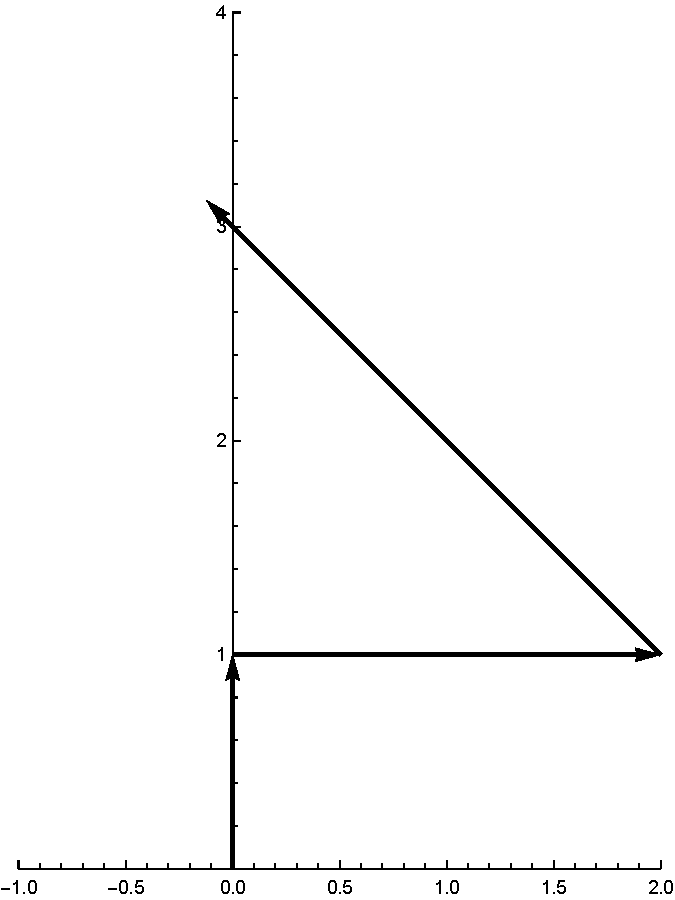
\includegraphics[scale=0.32]{1-16}
\end{figure}

From the plot we can see that the magnitude of the resultant vector is a little longer than $3\,mi$,
with a direction a little greater than $90^\circ$.

We can compute the exact values for magnitude and direction by determining the components of the resultant vector, as suggested for part (b).
The component in particular direction is the sum of the displacements in that direction for each leg of path.

For the x-direction, that's $0 + 2 + 3 \cdot \cos 135^\circ = 2 - \frac{\sqrt{3}}{2} \approx -0.12$.
For the y-direction, that's $1 + 0 + 3 \cdot \sin 135^\circ = 1 + \frac{\sqrt{3}}{2} \approx 3.12$.
The magnitude is $\sqrt{(2 - \frac{\sqrt{3}}{2})^2 + (1 + \frac{\sqrt{3}}{2})^2} \approx 3.12\,mi$,
while the direction is $\arctan(2 - \frac{\sqrt{3}}{2}, 1 + \frac{\sqrt{3}}{2}) \approx 92.23^\circ$.

The answer key gives $2.20^\circ$ W of N (same as $92.20^\circ$) as the answer.
You can account for the difference by using the approximate values for the x and y components
when computing the arctan.

\textbf{1-17} A bug starts at the center of a 12-inch phonograph record and crawls along a straight radial line to the edge.
While this is happening the record turns through an angle of $45^\circ$.
Draw a sketch of the situation and describe the magnitude and direction of the bug's displacement.

In the time that the bug travels a radial distance of $6\,in$, the phonograph record has rotated $45^\circ$,
so we can express the radial distance away from the center as a function of $\theta$: $r(\theta) = \frac{6}{45^\circ} \theta$.
This allows us to make a polar plot as follows:

\begin{figure}[h]
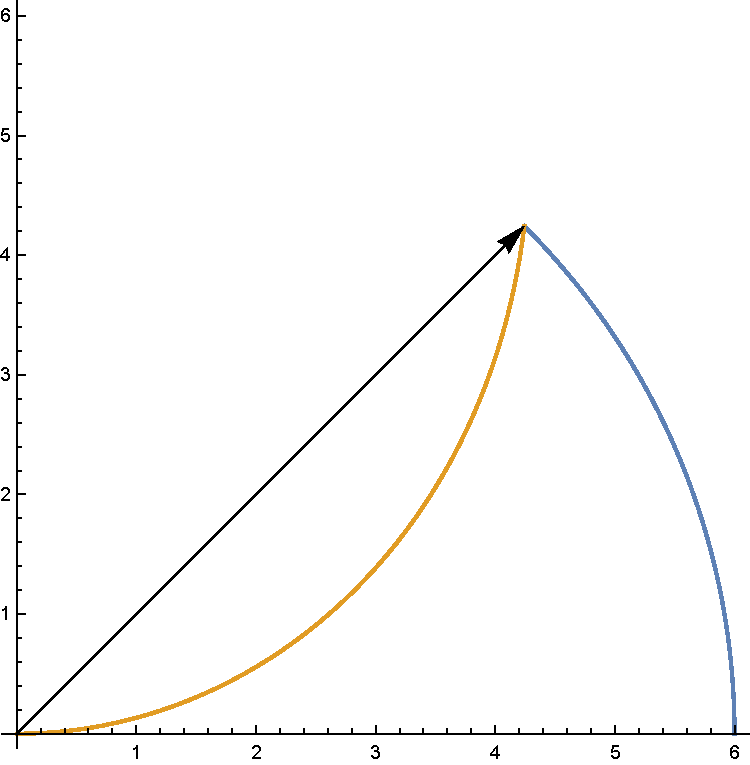
\includegraphics[scale=0.32]{1-17}
\end{figure}

The final displacement of the bug has a magnitude of $6\,in$ and a direction of $45^\circ$.

\textbf{1-18} A cave explorer is surveying a cave.  He follows a passage $100\,m$ straight east, then $50\,m$ in a direction $30^\circ$ west of north, then $150\,m$ at $45^\circ$ west of south.
After a fourth unmeasured displacement, he finds himself back where he started.
Using a scale drawing, determine the fourth displacement (magnitude and direction).

The path of the cave explorer is as follows:

\begin{figure}[h]
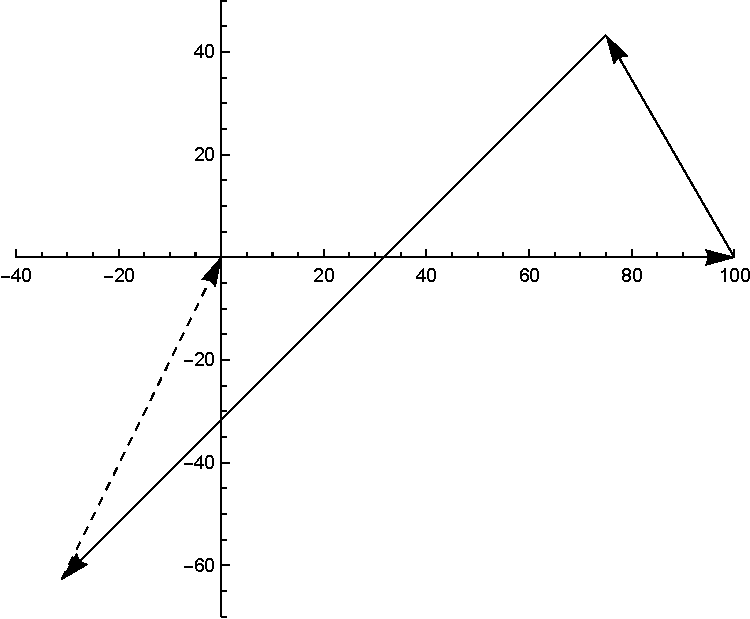
\includegraphics[scale=0.32]{1-18}
\end{figure}

We can determine the total displacement after the 3rd leg of the path by computing the total displacement in each direction.
The total x-displacement is $100 + 50 \cos 120^\circ + 150 \cos 225^\circ = 75 - 75 \sqrt{2} \approx -31.1$,
and the total y-displacment is $0 + 50 \sin 120^\circ + 150 \sin 225^\circ = -75 \sqrt{2} +25 \sqrt{3} \approx -62.8$.

It doesn't matter from where we started, since we are told that we return to that same point.
For the 4th leg to undo the displacements done by the first 3 legs,
we take the negative of cumulative displacement,
so the x-component of the 4th leg is 31.1 and its y-component is 62.8.
In vector form that's $\vec R_4 = 31.1 \hat i + 62.8 \hat j$.

The magnitude is $\sqrt{31.1^2+62.8^2} = 70.0\,m$, with direction $\arctan(31.1, 62.8) = 63.7^\circ$
(counterclockwise from the horizontal, the same as $90 - 63.7 = 26.3^\circ$ E of N).

\textbf{1-19} Find graphically the magnitude and direction of the vector sum of the three forces in Fig. 1-14 (of the book).
Use the polygon method.
Check the precision of your result by using the component method.

Let's first arrange the displacement vectors head-to-tail, as follows:

\begin{figure}[h]
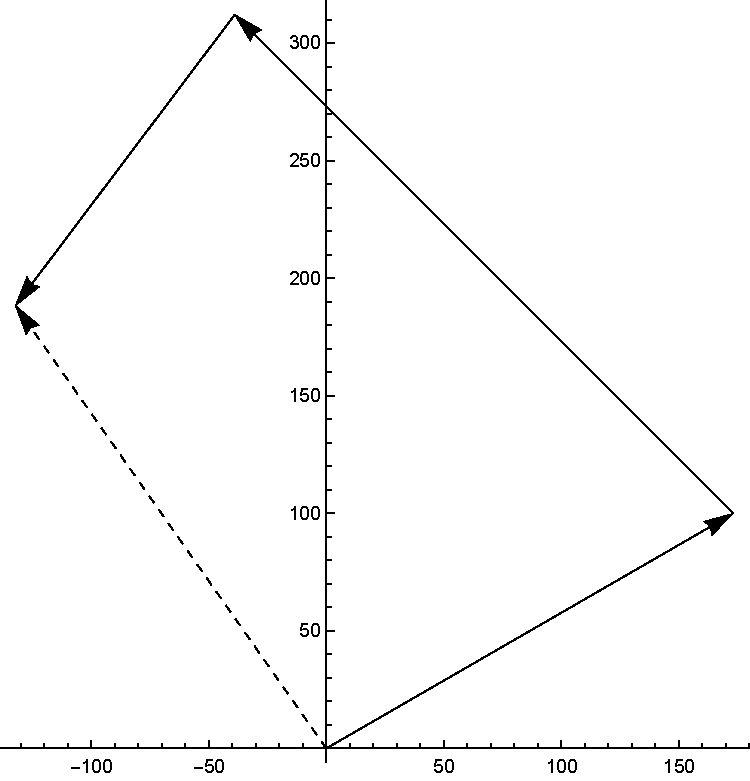
\includegraphics[scale=0.32]{1-19}
\end{figure}

As usual, to determine the components of the resultant vector, we sum the components of the vectors.
For the x-component, that's $200 \cos 30^\circ + 300 \cos 135^\circ + 155 \cos 233^\circ = -132.2$,
and for the y-component, that's $200 \sin 30^\circ + 300 \sin 135^\circ + 155 \sin 233^\circ = 188.3$.

The magnitude is $\sqrt{(-132.2)^2 + 188.3^2} = 230.1\,N$, with direction $\arctan(-132.2, 188.3) = 125.1^\circ$
(same as $180 - 125.1 = 54.9^\circ$ measured clockwise from negative horizonal).

\textbf{1-20} Find graphically the vector sum \textbf{A + B} and the vector difference \textbf{A - B} in Fig. 1-15 (of the book).

For the case of a sum of vectors, we arrange the vectors head-to-tail:

\begin{figure}[h]
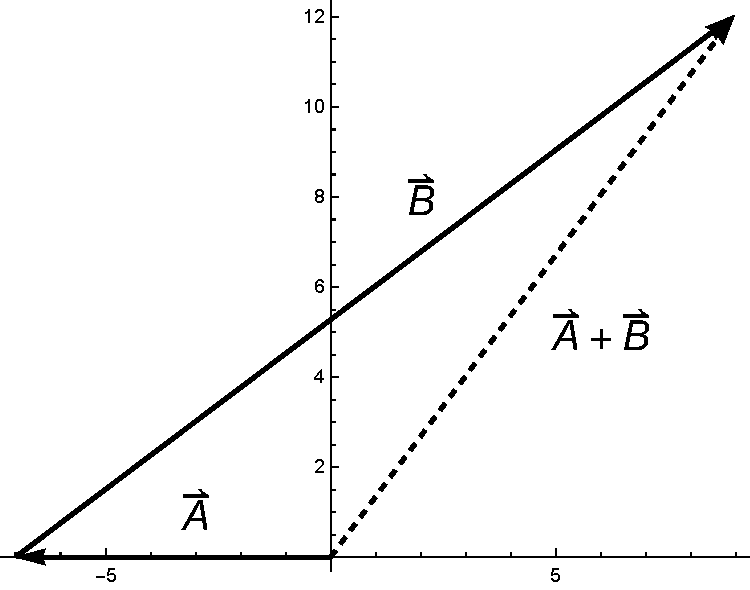
\includegraphics[scale=0.32]{1-20a}
\end{figure}
%\clearpage

For the difference of vectors, we arrange the vectors tail-to-tail:

\begin{figure}[h]
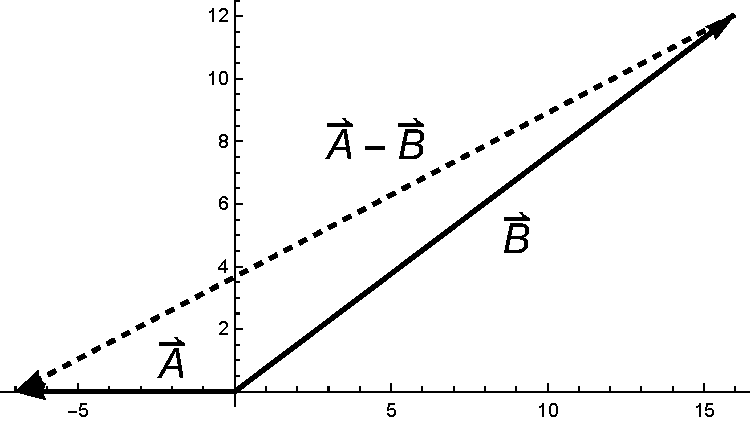
\includegraphics[scale=0.32]{1-20b}
\end{figure}

\textbf{1-21} Find the vector sum \textbf{A + B} and the vector difference \textbf{A - B} in Fig. 1-15 (of the book), using components.

The components of \textbf{A + B} are $-7 + 20 \cos 37^\circ = 9.0$ (in the x-direction) and $0 + 20 \sin 37^\circ = 12.0$ (in the y-direction).
The magnitude is $\sqrt{9^2 + 12^2} = 15.0\,N$, and the direction is $\arctan(9,12) = 53.3^\circ$.

The components of \textbf{A - B} are $-7 - 20 \cos 37^\circ = -23.0$ and $0 - 20 \sin 37^\circ = -12.0$.
The magnitude of the resultant is $\sqrt{(-23)^2 + (-12)^2} = 25.9\,N$, with direction $\arctan(-23, -12) = -152.3^\circ$
(same as $180 - 152.3 = 27.3^\circ$ below the --x-axis).

\textbf{1-22} Vector \textbf{A} is 2 in. long and is $60^\circ$ above the x-axis in the first quadrant.
Vector \textbf{B} is 2 in. long and is $60^\circ$ below the x-axis in the fourth quadrant.
Find graphically

a) the vector sum \textbf{A + B}, and

b) the vector differences \textbf{A - B} and \textbf{B - A}.

Here's the graph of vectors \textbf{A} and \textbf{B}:

\begin{figure}[h]
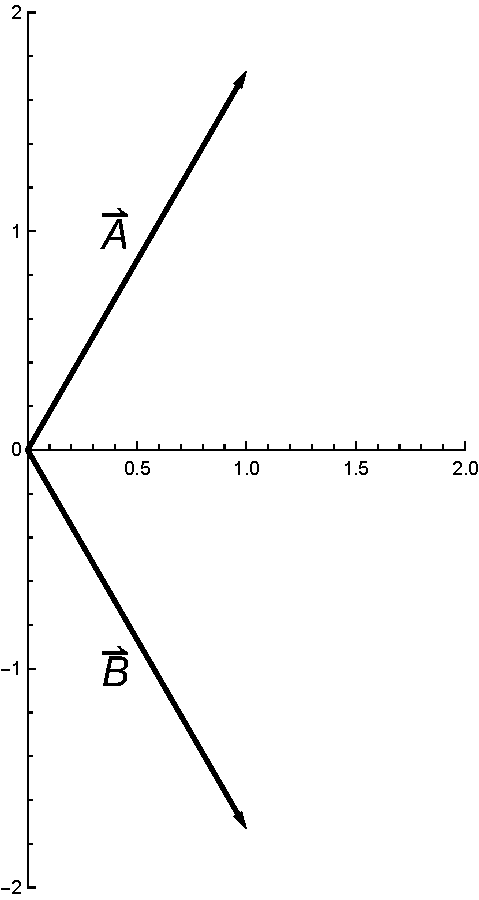
\includegraphics[scale=0.32]{1-22a}
\end{figure}

%\clearpage
For part (a), we arrange the vectors head-to-tail.  The resultant vector is:

\begin{figure}[h]
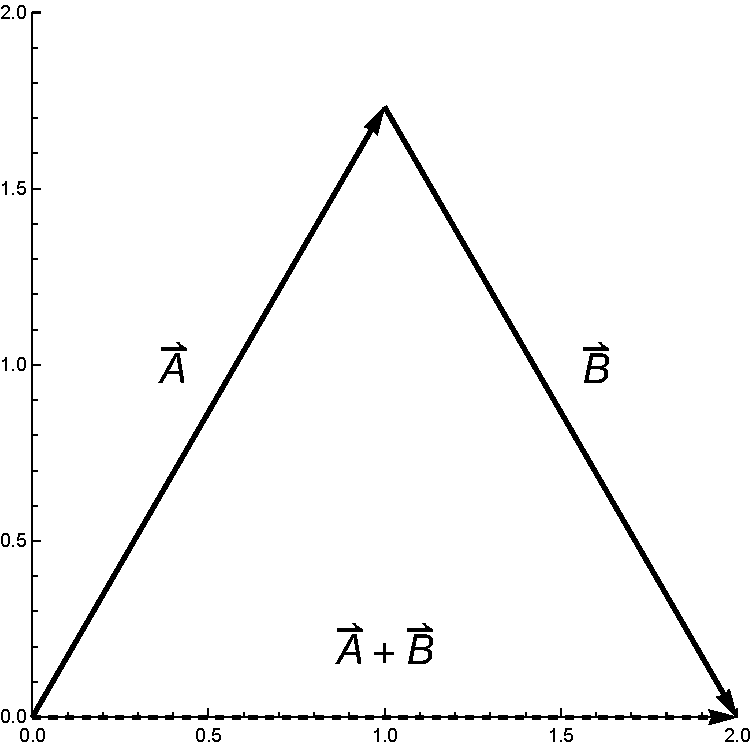
\includegraphics[scale=0.32]{1-22b}
\end{figure}

\clearpage

For part (b), we arrange the vectors tail-to-tail.
The resultant vector connects the heads:

%MJH - I could not get captions to work here.
\begin{figure}[h]
  \begin{minipage}[c]{0.4\textwidth}
    \centering
    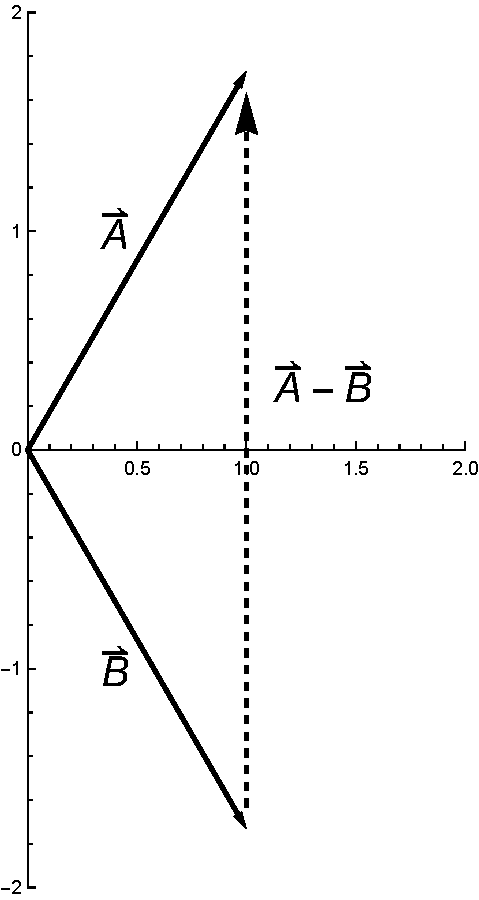
\includegraphics[scale=0.32]{1-22c}
  \end{minipage}
  \begin{minipage}[c]{0.4\textwidth}
    \centering
    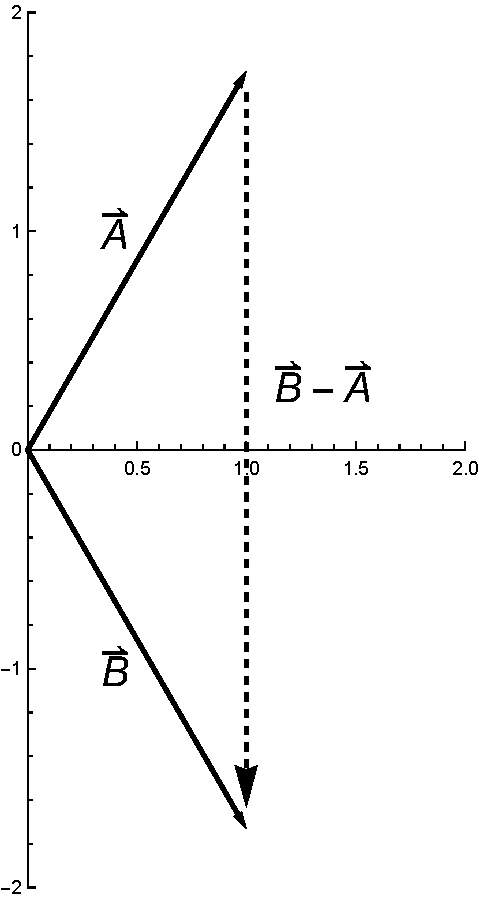
\includegraphics[scale=0.32]{1-22d}
  \end{minipage}
\end{figure}

\textbf{1-23} Obtain the vector sum and differences requested in Problem 1-22, using the method of components.

For the vector sum \textbf{A + B}, the x-component is $2 \cos 60^\circ + 2 \cos (-60^\circ) = 1 + 1 = 2$,
and the y-component is $2 \sin 60^\circ + 2 \sin (-60^\circ) = \sqrt{3} - \sqrt{3} = 0$.
The magnitude of the resultant is $\sqrt{2^2 + 0^2} = 2\,in$, with direction $\arctan(2,0) = 0^\circ$.

For the vector difference \textbf{A - B}, the x-component is $2 \cos 60^\circ - 2 cos (-60^\circ) = 1 - 1 = 0$,
and the y-component is $2 \sin 60^\circ - 2 \sin (-60^\circ) = \sqrt{3} - (-\sqrt{3}) = 2\sqrt{3}$.
The magnitude is $\sqrt{0^2 + (2\sqrt{3})^2} = 2\sqrt{3}\,in$, with direction $\arctan(0, 2\sqrt{3}) = 90^\circ$.

For the vector difference \textbf{B - A}, the x-component is $2 \cos (-60^\circ) - 2 cos 60^\circ = 1 - 1 = 0$,
and the y-component is $2 \sin (-60^\circ) - 2 \sin 60^\circ = -\sqrt{3} - \sqrt{3} = -2\sqrt{3}$.
The magnitude is $\sqrt{0^2 + (-2\sqrt{3})^2} = 2\sqrt{3}\,in$, with direction $\arctan(0, -2\sqrt{3}) = -90^\circ$.

\textbf{1-24} Vector \textbf{A} has components $A_x$ = 2 cm, $A_y$ = 3 cm,
and vector \textbf{B} has components $B_x$ = 4 cm, $B_y$ = -2 cm.
Find

a) the components of the vector sum \textbf{A + B};

b) the magnitude and direction of \textbf{A + B};

c) the components of the vector difference \textbf{A - B};

d) the magnitude and direction of \textbf{A - B}.

For (a), the x-component is 2 + 4 = 6, and the y-component is 3 + (-2) = 1.

For (b), the magnitude is $\sqrt{6^2+1^2} = \sqrt{37} \approx 6.1$\,cm,
and the direction is $\arctan(6,1) = 9.5^\circ$.

For (c), the x-component is 2 - 4 = -2, and the y-component is 3 - (-2) = 5.

For (d), the magnitude is $\sqrt{(-2)^2 + 5^2} = \sqrt{29} \approx 5.4$\,cm,
and the direction is $\arctan(-2, 5) = 111.8^\circ$.

\textbf{1-25} A car drives 5 mi east, then 4 mi south, then 2 mi west.
Find the magnitude and direction of the resultant displacement.

The x-component is 5 + 0 - 2 = 3, and the y-component is 0 - 4 + 0 = -4.
The magnitude is $\sqrt{3^2+(-4)^2} = 5$\,mi, and the direction is $\arctan(3,-4) = -53.1^\circ$
(same as $53.1^\circ$ south of east).

\textbf{1-26} A sailboat sails 2 km east, then 4 km southeast, then an additional distance in an unknown direction.
Its final position is 5 km directly east of the starting point.
Find the magnitude and direction of the third leg of the journey.

We are told the final displacement of the sailboat.
The final displacement is the sum of the displacements from each leg,
so we can work backwards to find the displacement due to the third leg.

The displacement in the x-direction is $2 + 4 \cos (-45^\circ) + x = 5$;
solving for x yields the value $3 - 2\sqrt{2} \approx 0.172$.

The displacement in the y-direction is $0 + 4 \sin (-45^\circ) + y = 0$;
solving for y yields the value $2 \sqrt{2} \approx 2.828$.

We have each component, so we can find the magnitude and direction in the normal way.
The magnitude is $\sqrt{(3 - 2\sqrt{2})^2 + (2\sqrt{2})^2}$ = 2.83\,km,
having a direction $\arctan (3-2\sqrt{2}, 2\sqrt{2})$ = $86.5^\circ$
(same as $90 - 86.5 = 3.5^\circ$ east of north).

The answer booklet gives $3.4^\circ$ east of north as the answer,
which is the result obtained if you compute the arctan using component values having fewer than 3 digits of precision.

\textbf{1-27} Vector \textbf{M}, of magnitude 5\,cm, is at $36.9^\circ$ counterclockwise from the +x-axis.
It is added to vector \textbf{N}, and the resultant is a vector of magnitude 5\,cm, at $53.1^\circ$ counterclockwise from the +x-axis.
Find\newline
a) the components of \textbf{N};\newline
b) the magnitude and direction of \textbf{N}.

We are told that \textbf{R} = \textbf{M + N}, so \textbf{N} is just the vector difference \textbf{R - M}.
The x-component of \textbf{N} is $5 \cos 53.1^\circ - 5 \cos 36.9^\circ$ = -1\,cm,
and the y-component is $5 \sin 53.1^\circ - 5 \sin 36.9^\circ$ = 1\,cm.

The magnitude is $\sqrt{(-1)^2 + 1^2}$ = 1.41\,cm, with direction $\arctan(-1,1)$ = $135^\circ$.

The exact angles are $2\,\arctan \frac{1}{2}$ (for $53.1^\circ$)
and $\frac{\pi}{2} - 2\,\arctan \frac{1}{2}$ (for $36.9^\circ$).

\textbf{1-28} A vector \textbf{A} of length 10 units makes an angle of $30^\circ$ with a vector \textbf{B}
of length 6 units.
Find the magnitude of the vector difference \textbf{A - B} and the angle it makes with vector \textbf{A}:\newline
a) by the triangle method;\newline
b) by the method of rectangular resolution.

Here's a diagram of the vectors:

\begin{figure}[h]
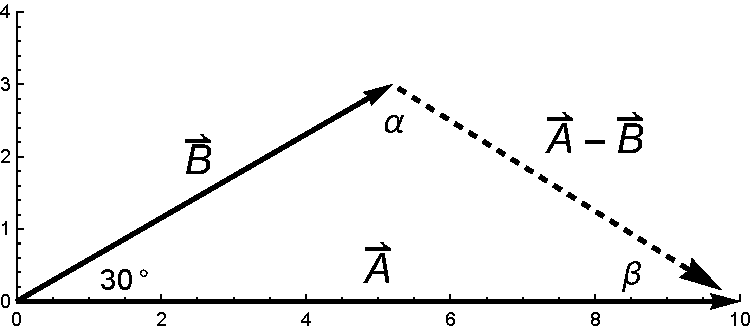
\includegraphics[scale=0.32]{1-28}
\end{figure}

The problem is asking us to find the angle between \textbf{A} and \textbf{A - B}; that's angle $\beta$ in the diagram,
the angle opposite vector \textbf{B}.

For part (a), we can use the Law of Cosines to find the length of the difference vector (call it \textbf{C}), and then use the Law of Sines to
find the angle.

Per the Law of Cosines, the length C = $\sqrt{A^2 + B^2 - 2 A B \cos 30^\circ}$ =
$\sqrt{10^2 + 6^2 - 2\cdot10\cdot6\cdot\cos 30^\circ}$ = $\sqrt{136 - 60 \sqrt{3}} \approx 5.66$.

Per Law of Sines, the relationship among the lengths and angles is $\frac{\sin \beta}{B} = \frac{\sin 30^\circ}{C}$,
so solving for $\beta$, that's $\beta = \arcsin \left( \frac{B \cdot \sin 30^\circ}{C} \right)$ =
$\arcsin \left( \frac{6 \cdot \sin 30^\circ}{5.66} \right)$ = $32.0^\circ$.

For part (b), we use vector composition.
The x-component of the vector difference is 10 - 6 $\cos 30^\circ$ = 10 - 3 $\sqrt{3}$ $\approx$ 4.8,
and the y-component is 0 - 6 $\sin 30^\circ$ = -3.
It has magnitude is $\sqrt{4.8^2 + (-3)^2}$ = 5.66 and direction $\arctan (4.8,-3)$ = $-32.0^\circ$.
That angle value is measured from the positive +x-axis, but want the interior angle of the
triangle ($\beta$ in the diagram above), so that's $32.0^\circ$.

\textbf{1-29} Two vectors \textbf{A} and \textbf{B} have the same magnitude.
Under what circumstances does the vector sum \textbf{A + B} have the same magnitude as \textbf{A} and \textbf{B}?
When does the vector difference \textbf{A - B} have this magnitude?

The vectors form the sides of an equilateral triangle.  The vector sum \textbf{A + B} looks like this:

\begin{figure}[h]
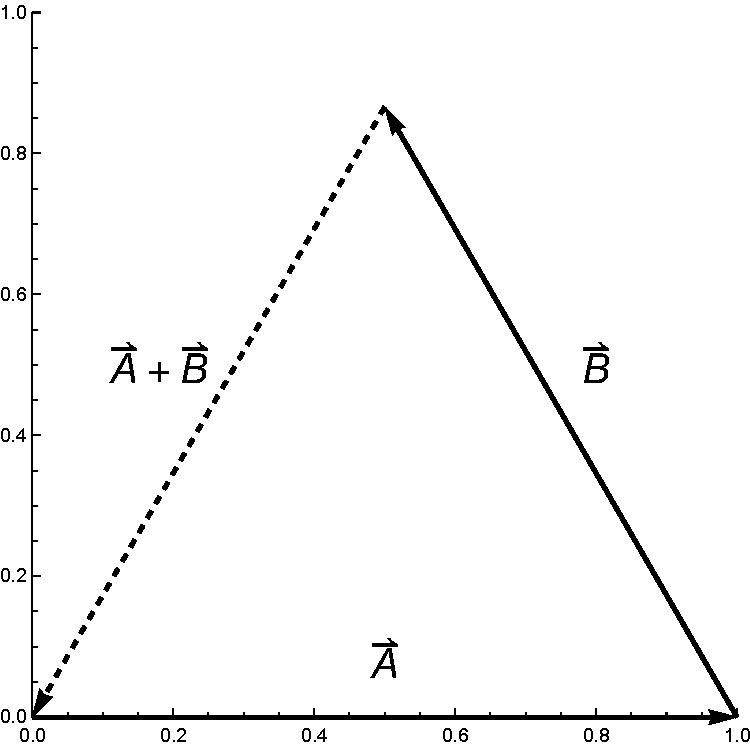
\includegraphics[scale=0.32]{1-29a}
\end{figure}

The interior angles are all $60^\circ$, so the direction of vector \textbf{B}, measured from the +x-axis,
would be $120^\circ$.  We can prove this mathematically using the Law of Cosines.
All the magnitudes are the same, so we can write $A^2 = A^2 + A^2 - 2 A A \cos \theta$.
Dividing by $A^2$ and simplifying, that's $2 \cos \theta = 1$, so $\theta = \arccos (1/2) = 60^\circ$.

For the vector difference \textbf{A - B}, we arrange the vectors tail-to-tail:

\begin{figure}[h]
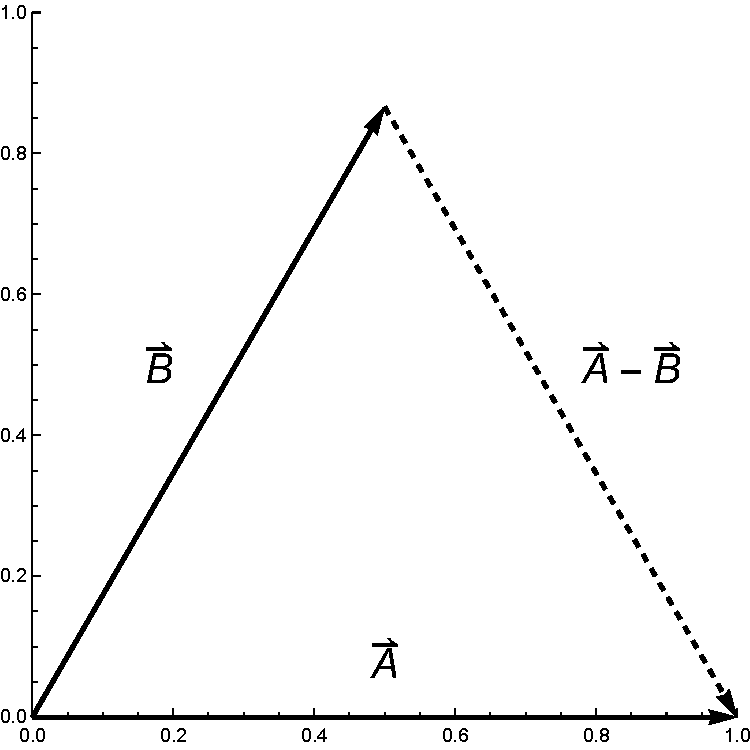
\includegraphics[scale=0.32]{1-29b}
\end{figure}

Here the direction for \textbf{B} is the same as interior angle, $60^\circ$.

\textbf{1-30} Given two vectors \textbf{A} = $2\hat i + 3\hat j$ and \textbf{B} = $\hat i -2\hat j$,
obtain the following:\newline
a) Find the magnitude of each vector.\newline
b) Write an expression for the vector sum, using unit vectors.\newline
c) Find the magnitude and direction of the vector sum.\newline
d) Write an expression for the vector difference \textbf{A - B}, using unit vectors.\newline
e) Find the magnitude and direction of the vector difference \textbf{A - B}.

The magnitude of \textbf{A} is $\sqrt{2^2+3^2}$ = $\sqrt{13}$,
and \textbf{B} is $\sqrt{1^2 + (-2)^2}$ = $\sqrt{5}$.

The x-component of the sum is 2 + 1 = 3, and the y-component is 3 - 2 = 1.
Written in vector form, that's \textbf{A + B} = $3 \hat i + \hat j$.

The magnitude of the vector sum is $\sqrt{3^2 + 1^2}$ = $\sqrt{10}$,
and its direction is $\arctan(3,1)$ = $18.4^\circ$.

The x-component of the difference is 2 - 1 = 1, and the y-component is 3 - (-2) = 5.
In vector form that's \textbf{A - B} = $\hat i + 5 \hat j$.

The magnitude of the difference is $\sqrt{1^2 + 5^2}$ = $\sqrt{26}$,
and the direction is $\arctan(1,5)$ = $78.7^\circ$.

\textbf{1-31} Given two vectors \textbf{A} = $2 \hat i + 3 \hat j + 4 \hat k$
and \textbf{B} = $\hat i - 2 \hat j + 3 \hat k$, obtain the following:\newline
a) Find the magnitude of each vector.\newline
b) Write an expression for the vector sum, using unit vectors.\newline
c) Find the magnitude of the vector sum.\newline
d) Write an expression for the vector difference \textbf{A - B}, using unit vectors.\newline
e) Find the magnitude of the vector difference \textbf{A - B}.
Is this the same as the magnitude of \textbf{B - A}?  Explain.

The magnitude of \textbf{A} is $\sqrt{2^2 + 3^2 + 4^2}$ = $\sqrt{29}$,
and for \textbf{B} it's $\sqrt{1^2 + (-2)^2 + 3^2}$ = $\sqrt{14}$.

The components of the vector sum are $2+1 = 3$, $3-2=1$, and $4+3=7$.
The vector form of the sum is \textbf{A + B} = $3 \hat i + \hat j + 7 \hat k$.

The magnitude of the vector sum is $\sqrt{3^2 + 1^1 + 7^2}$ = $\sqrt{59}$.

The components of the vector difference are $2-1=1$, $3-(-2)=5$, and $4-3=1$.
In vector form that's \textbf{A - B} = $\hat i + 5 \hat j + \hat k$.

The magnitude of the vector difference \textbf{A - B} is $\sqrt{1^2 + 5^2 + 1^2}$ = $\sqrt{27}$ = $3 \sqrt{3}$.
This is the same as the magnitude of \textbf{B - A}, since it differs from \textbf{A - B} only in its direction.

\textbf{1-32} Write out a multiplication table for the scalar products of all possible pairs of unit vectors,
such as \textbf{i $\cdot$ i = ?}, \textbf{i $\cdot $ j = ?}, and so on.

Here's a table of scalar products:

\begin{figure}[h]
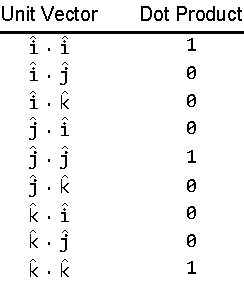
\includegraphics[scale=1.0]{1-32}
\end{figure}

\clearpage

\textbf{1-33} Write out a multiplication table for the vector products of all possible pairs of unit vectors,
such as \textbf{i $\times$ i = ?}, \textbf{i $\times $ j = ?}, and so on, using a righthanded coordinate system.

Here's a table of vector products:

\begin{figure}[h]
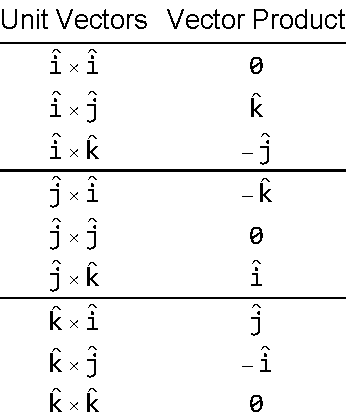
\includegraphics[scale=0.8]{1-33}
\end{figure}

\noindent
\textbf{1-34} Find the angle between the diagonal of a cube and an edge,
using a method similar to that in the example of Sec.\ 1-8.
Is this the same as the angle between the diagonal of a face and an edge?

The dot product \textbf{A $\cdot$ B} is the sum of the product of like components,
$A_x \cdot B_x + A_y \cdot B_y + A_z \cdot B_z$.
Here, \textbf{A} is the diagonal of a cube, $\hat i + \hat j + \hat k$.
We can use any edge, so let \textbf{B} = $\hat i$.
The dot product would have as its scalar value $1 \cdot 1 + 1 \cdot 0 + 1 \cdot 0 = 1$.

But the dot product is defined as \textbf{A $\cdot$ B} = $\abs{A} \abs {B} \cos \theta$.
The magnitude of \textbf{A} is $\abs{A} = \sqrt{1^2 + 1^2 + 1^2} = \sqrt{3}$,
while the magnitude of \textbf{B} is $\abs{B} = \sqrt{1^2} = 1$.
Equating then dividing by the magnitudes, that's $\cos \theta = \frac{1}{\sqrt{3} \cdot 1}$,
so $\theta = \arccos \frac{1}{\sqrt{3}} = 54.7^\circ$.

This value is different from the angle between the diagonal of a face and an edge,
which would be $45^\circ$.

\vspace{\baselineskip}

\noindent
\textbf{1-35} Find the scalar product of the two vectors given in Problem 1-31.

\textbf{A} = $2 \hat i + 3 \hat j + 4 \hat k$, and \textbf{B} = $\hat i - 2 \hat j + 3 \hat k$,
so all we need to do is take the sum of the product of like components.
\textbf{A} $\cdot$ \textbf{B} = $2 \cdot 1 + 3 \cdot (-2) + 4 \cdot 3$ = 2 - 6 + 12 = 8.

\vspace{\baselineskip}

\noindent
\textbf{1-36} Find the vector product of the two vectors given in Problem 1-31.
What is the magnitude of this vector product?

Let \textbf{C = A $\times$ B}.  We compute the components per eqn.\ (1-29) in the book.
$C_x = A_y B_z - A_z B_y = 3 \cdot 3 - 4 \cdot (-2) = 9 + 8 = 17$.
$C_y = A_z B_x - A_x B_z = 4 \cdot 1 - 2 \cdot 3 = 4 - 6 = -2$.
$C_z = A_x B_y - A_y B_x = 2 \cdot (-2) - 3 \cdot 1 = -4 - 3 = -7$.

In vector form, that's \textbf{C} = $17 \hat i -2 \hat j -7 \hat k$.
The magnitude is $\sqrt{17^2 + (-2)^2 + (-7)^2} = \sqrt{342}$.

\vspace{\baselineskip}

\noindent
\textbf{1-37} Obtain a unit vector perpendicular to the two vectors given in Problem 1-31.

To obtain the unit vector, we divide the vector cross product by its magnitude:
$\pm \frac{1}{\sqrt{342}} (17 \hat i -2 \hat j -7 \hat k)$.
Here we use $\pm$ to indicate that either direction qualifies as a (unit) vector
perpendicular to the plane of the two vectors \textbf{A} and \textbf{B}.

\vspace{\baselineskip}

\noindent
\textbf{1-38} Find the angle between the two vectors \textbf{A} = $3 \hat i + 4 \hat j + 5 \hat k$
and \textbf{B} = $3 \hat i + 4 \hat j - 5 \hat k$.

We use the formula for the dot product:
$A B \cos \theta$ = \textbf{A $\cdot$ B} = $A_x B_x + A_y B_y + A_z B_z$.
Here the dot product is $3 \cdot 3 + 4 \cdot 4 + 5 \cdot (-5)$ = 9 + 16 - 25 = 0,
so $\theta = \arccos 0 = 90^\circ$.

\vspace{\baselineskip}

\noindent
\textbf{1-39} Consider the two repeated vector products \textbf{i $\times$ (i $\times$ j)}
and \textbf{(i $\times$ i) $\times$ j}.\newline
a) Are these two products equal?\newline
b) Can you generalize this result for this type of repeated product?

No, they're not equal:  \textbf{i $\times$ (i $\times$ j)} =
\textbf{i $\times$ k} = \textbf{-j},
but \textbf{(i $\times$ i) $\times$ j} = \textbf{0 $\times$ j} = 0.
The vector cross product is not associative, so in general they won't be equal.

\vspace{\baselineskip}

\noindent
\textbf{1-40} Prove that for any three vectors \textbf{A}, \textbf{B}, and \textbf{C},
\textbf{A $\cdot$ (B $\times$ C)} = \textbf{(A $\times$ B) $\cdot$ C}.

Let \textbf{D = B $\times$ C}.  Then $D_x = B_y C_z - B_z C_y$, $D_y = B_z C_x - B_x C_z$, and $D_z = B_x C_y - B_y C_x$.
The scalar product is \textbf{A $\cdot$ (B $\times$ C) = A $\cdot$ D} = $A_x D_x + A_y D_y + A_z D_z$ =
$A_x (B_y C_z - B_z C_y)$ + $A_y (B_z C_x - B_x C_z)$ + $A_z (B_x C_y - B_y C_x)$ =
$A_x B_y C_z - A_x B_z C_y + A_y B_z C_x - A_y B_x C_z + A_z B_x C_y - A_z B_y C_x$.

We now group according to components of \textbf{C}:
$A_y B_z C_x - A_z B_y C_x + A_z B_x C_y - A_x B_z C_y + A_x B_y C_z - A_y B_x C_z$ =
$(A_y B_z - A_z B_y) C_x + (A_z B_x - A_x B_z) C_y + (A_x B_y - A_y B_x) C_z$.
But the parenthesized terms are just the components \textbf{A $\times$ B},
and the respective products are the dot product, \textbf{(A $\times$ B) $\cdot$ C}.

\vspace{\baselineskip}
\noindent
Study Guide - Chapter 1 Quiz

\vspace{\baselineskip}
\noindent
\textbf{1} Find the sum (\textbf{C}) and difference (\textbf{D}) of the vectors \textbf{A} and \textbf{B}
shown in the Fig.\,1-14.

Vector \textbf{A} has components (7, 0) and \textbf{B} has components $15 (\cos 37^\circ, \sin 37^\circ)$.
Vector \textbf{C} is just the component-wise sum, $(7 + 15 \cos 37^\circ, 15 \sin 37^\circ)$ = $(19.0, 9.0)$.
The magnitude is $\sqrt{19^2 + 9.0^2}$ = 21.0, and the angle is $\arctan(19.0, 9.0)$ = $25.4^\circ$.

Difference vector \textbf{D} = \textbf{A} - \textbf{B} = $(7 - \cos 37^\circ, -15 \sin 37^\circ)$
= (-5.0, -9.0).  The magnitude is $\sqrt{(-5.0)^2 + (-9.0)^2}$ = 10.3, with angle
$\arctan(-5.0, -9.0)$ = $-118.9^\circ$  (same as $241.1^\circ$ measured counter-clockwise).

\vspace{\baselineskip}
\noindent
\textbf{2} Two forces \textbf{$F_1$} and \textbf{$F_2$} act on a body at the origin as shown in Fig.\,1-15.
Find a third force \textbf{$F_3$} acting at the origin such that the total force acting on the body is zero.

We have $F_1$ = $10 (\cos 30^\circ, \sin 30^\circ)$, and $F_2$ = $5 (\cos (-45^\circ), \sin (-45^\circ))$.
We want $F_3$ = -$(F_1 + F_2)$ = -$(10 \cos 30^\circ + 5 \cos (-45^\circ), 10 \sin 30^\circ +5 \sin (-45^\circ))$
= (-12.2, -1.46).  The magnitude is $\sqrt{(-12.2)^2 + (-1.46)^2}$ = 12.2\,N,
with the angle equal to $\arctan(-12.2, -1.46)$ = $-173^\circ$ (same as $187^\circ$ measured counter-clockwise).

\clearpage

% 2018-06-27

Chapter 2

\textbf{Questions}

\vspace{\baselineskip}

\noindent
\textbf{2-1} Can a body be in equilibrium when only one force acts on it?

No, because then there would be a non-zero net force, so the body would be accelerating.
(I am interpreting ``equilibrium" here to mean ``no net force".)

\vspace{\baselineskip}

\noindent
\textbf{2-2} A helium balloon hovers in midair, neither ascending nor descending.
Is it in equilibrium?
What forces act on it?

Yes, the balloon is in equilibrium, because it is not accelerating.
The forces acting on the balloon are the force of gravity (pulling it down)
and the buoyant force (pushing it up).
Here these forces exactly cancel, so there is no net force and hence no acceleration.

\vspace{\baselineskip}

\noindent
\textbf{2-3} If the two ends of a rope in equilibrium are pulled with forces of equal magnitude
and opposite direction, why is the total tension in the rope not zero?

The purpose of a rope is to transmit a force.
(And the purpose of a pulley is to change the direction of a force.)
No \textit{net} force doesn't mean no force at all, it only means that the sum of the forces is zero.
That there is tension in the rope \textit{means} that there are forces acting on the rope,
and in opposite directions.
But saying that the total net force is zero, is not the same as saying that there is no tension.

\vspace{\baselineskip}

\noindent
\textbf{2-4} A horse is hitched to a wagon.
Since the wagon pulls back on the horse just as hard as the horse pulls on the wagon,
why doesn't the wagon remain in equilibrium, no matter how hard the horse pulls?

Because these describe different forces, acting on different objects.
The horse pulls on the wagon, so the wagon feels a force.  Full stop.
The fact that that force is part of a reaction pair is irrelevant,
because the other member of the pair acts on the horse, not the wagon.

\vspace{\baselineskip}

\noindent
\textbf{2-5} A clothesline is hung between two poles, and then a shirt is being hung near the center.
No matter how tightly the line is stretched, it always sags a little at the center.
Explain why.

There is a downward force on the first shirt, due to gravity.
If the shirt is in equilibrium, then there must be some other upward force.
The upward force is coming from the clothesline.
The only way there can be an upward force is if the tension in the line has both upward and sideways components,
which means there must be a bend in the rope.  (The tension is directed at an angle to the horizontal.)
Stretching the line more tightly would only increase the horizontal component of the tension,
but the downward force due to the weight of the shirt doesn't change,
and so the vertical component of the tension would not change.

(The forces here form the sides of a triangle.
The vertical side has a constant length,
because its length is whatever it needs to be for the shirt to be in equilibrium.
The horizonal side grows in length as the horizontal component of the tension is increased,
and the hypotenuse grows to compensate.)

\vspace{\baselineskip}

\noindent
\textbf{2-6} A man sits in a chair that is suspended from a rope.
The rope passes over a pulley suspended from the ceiling and the man holds the other end
of the rope in his hands.
What is the tension in the rope, and what force does the chair exert on the man?

Intuitively, we know that if you were suspended from a single rope attached to the ceiling,
that the tension in the rope would be equal to your weight.
If we were to hang two pieces of rope from the ceiling, and you suspended yourself by
hanging onto both ropes (as a gymnast, say), then your weight would be distributed between
both ropes and so each rope would have a tension equal to half of your weight.

If the man is pulling down on the rope (on one side of the pulley) with his hands,
then per Newton's third law, the rope is pulling up on the man.
If the tension in the rope accounts for half of his weight,
then the chair must account for the other half of his weight, since the man is in equilibrium.

That's our intuition, but let's confirm out intuition with math (because, hey, math is awesome).
The forces on the man are the tension in the rope (T, pulling him up), the normal force of the chair
(N, pushing him up), and the force of gravity (mg, pulling him down).
The man is in equilibrium, so we have T + N - mg = 0.

The forces on the chair are the normal force of the man (N, directed down), and the tension
of the rope (T, pulling the chair up).
Note that the tension is the same everywhere in the rope.  So that's T - N = 0.

Adding these two equations together, we have T + N - mg + T - N = 0, which is 2T = mg and so T = $\frac{1}{2}$mg,
which confirms our intuition (see, I told you math was awesome).  The normal force is N = T, so N is also $\frac{1}{2}$mg.

The normal force is a third-law pair, so the normal force of the chair on the man is the same as the normal force
of the man on the chair, just in the opposite direction.  Note that the normal force is a \textit{constraint force},
so it adjusts as required to preserve Newton's laws.
Here the man is pulling down on the rope, so the rope is pulling up on the man, and this makes the normal force less
than it would be otherwise, were the man simply sitting in the chair.

\vspace{\baselineskip}

\noindent
\textbf{2-7} How can pushing down on a bicycle pedal make the bicycle move \textit{forward}?

The gears change the direction of the force (not unlike what a pulley does).
The chain transmits the force to the back wheel, creating a torque, which causes the wheel to rotate.
There is friction between the wheel and the road.
(There is no relative motion between the wheel and the road at the point of contact, so this static friction.)
The wheel is pushing against the road.
Per the third law, there is a reaction force, from the road to the wheel.
This is the force that propels the bicycle forward.

\vspace{\baselineskip}

\noindent
\textbf{2-8} A car is driven up a steep hill at constant speed.
Discuss all the forces acting on the car; in particular, what pushes it up the hill?

There is a normal force from the road to the car, in a direction perpendicular to the road.
There is the force of gravity on the car, directed downwards, towards the center of the earth.

There is one more force acting on the car.
As with the bicycle in 2-7, the wheel pushes against the road, so the road pushes against the wheel, per the third law.

If you decompose the force due to gravity, there is a component directed down, perpendicular from the road.
This force is exactly balanced by the normal force (there is no acceleration in the perpendicular direction).
There is also a component directed backwards, parallel to the road.  This force is exactly balanced by the frictional force
(the car is traveling at constant velocity, so there is no acceleration, hence the forces in the parallel direction must also be in balance).

\vspace{\baselineskip}

\noindent
\textbf{2-9} Can the coefficient of friction ever be greater than unity?
If so, give an example; if not, explain why not.

The frictional force is proportional to the normal force.
For the coefficient of friction to be greater than unity, the frictional force would need to be greater than the normal force.
This can happen if the surfaces were sticky (perhaps they're attached using Velcro), or made from rubber or something.

\vspace{\baselineskip}

\noindent
\textbf{2-10} A block rests on an inclined plane with enough friction to prevent sliding down.
To start the block moving, is it easier to push it up the plane, down the plane, or sideways?  Why?

It would require the least amount of force to get the block moving by pushing the block down the plane.

Static friction force is a constraint force, meaning that it adjusts, enough to exactly balance the force
on the object parallel to the surface, but only up to the limit of $\mu_s \cdot$ \textbf{N}.
There is a component of the gravitational force directed down the ramp, so this gives us a kind of head start.
We would only need to apply an amount of force equal to the difference between the maximum frictional force
and the component of gravity directed down the ramp.

Pushing in other directions would require more force.
Were we to push the block up the ramp, we would first have to overcome the gravitational force,
and then overcome the maximum frictional force (which would now be pointed the other way, down the ramp).
If we were to push sideways, we would need to overcome the maximum frictional force.

\vspace{\baselineskip}

\noindent
\textbf{2-11} In pushing a box up a ramp, is it better to push horizontally or to push parallel to the ramp?

It's better to push parallel to the ramp.  A horizontal push force has an upward component, parallel to the ramp,
and another downward component, perpendicular to the ramp.  The perpendicular component would add to the component
of the gravitational force also perpendicular to the ramp, which would only increase the normal force.

The work done on an object (here, on a box, to raise it higher) is the scalar product of the force
and the displacement, so any forces on the object not along the displacement vector are wasted.
Things are even worse if there is friction, because increasing the normal force would increase the maximum
frictional force, and you'd have to increase the parallel component of the force to compensate.

If you push the box parallel to the ramp, the normal force is due to gravity alone, so the maximum frictional force
would be less, and none of the force would be wasted.

\vspace{\baselineskip}

\noindent
\textbf{2-12} In stopping a car on an icy road, is it better to push the brake pedal hard enough to ``lock"
the wheels and make them slide, or to push gently so the wheels continue to roll?  Why?

It's better to gently push, so the wheels continue to roll.  If the wheels were sliding against the road,
then the relative velocity would be positive, and the frictional force would be kinetic.
Kinetic friction has a lower coefficient than static friction, so the frictional force would be less,
and there would be less deceleration.

\vspace{\baselineskip}

\noindent
\textbf{2-13} When one stands with bare feet in a wet bathtub, the grip feels fairly secure,
and yet a catastrophic slip is quite possible.
Discuss this situation with respect to the two coefficients of friction.

Static friction is a constraint force, so it adjusts but only up to a limit.
If you were to shift your stance a little but with enough force to overcome the force of static friction,
resulting in relative motion, then the frictional force would become kinetic.
Suddenly there is a positive net force, because the force of friction is now less then the shifting force,
so your feet would accelerate.
It might be the case the wet surface acts as a lubricant, making the kinetic friction small compared to static friction.
This would exaggerate the effect of a slip (your feet would accelerate quickly), so you wouldn't have time to react,
making a fall more likely.

\vspace{\baselineskip}

\noindent
\textbf{2-14} The horrible squeak made by a piece of chalk held against a blackboard at the wrong angle results
from an alternate sticking and slipping of the chalk against the blackboard.
Interpret this phenomenon in terms of the two coefficients of friction.
Can you think of other examples of ``slip-stick" behavior?

As soon as the chalk slips, the frictional force is kinetic and now the chalk accelerates.
But suppose it happens to hit a patch of the blackboard with a little more friction,
and so the chalk decelerates, like screeching tires.

Another example: suppose you're on a bicycle heading fast downhill, but then jam on the brakes.
You're still moving, but the bicycle tires slide across the pavement, not unlike how the chalk slides across the blackboard.

\vspace{\baselineskip}

\textbf{Problems}

\vspace{\baselineskip}

\noindent
\textbf{2-1} \newline
a) Find graphically the horizontal and vertical components of a 40-N force the direction
of which is $50^\circ$ above the horizontal to the right.  Let 1 cm = 5 N. \newline
b) Check your results by calculating the components.

Here's a plot of the force vector:

\begin{figure}[h]
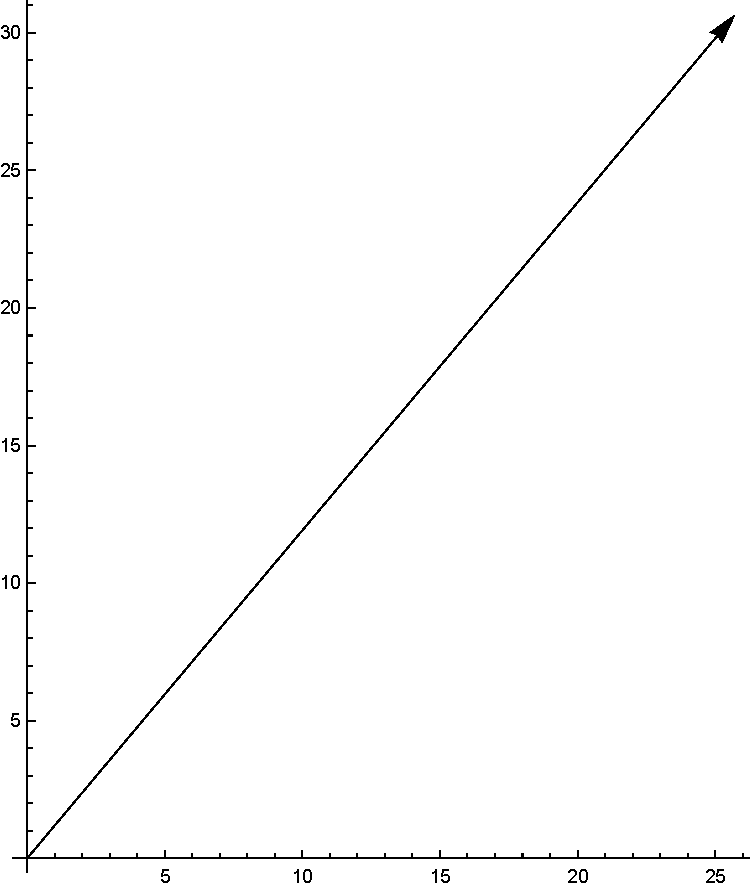
\includegraphics[scale=0.3]{2-1}
\end{figure}

The vector is $\vec F$ = 40 ($\cos 50^\circ,\sin 50^\circ$) = (25.7 N, 30.6 N).
\clearpage

\noindent
\textbf{2-2} A box is pushed along the floor as in Fig. 2-1b (in the book) by a force
of 40 N making an angle of $30^\circ$ with the horizontal.
Using a scale of 1 cm = 5 N, find the horizontal and vertical components of the force by the graphical
method.
Check your results by calculating the components.

Here's a plot of the force vector:

\begin{figure}[h]
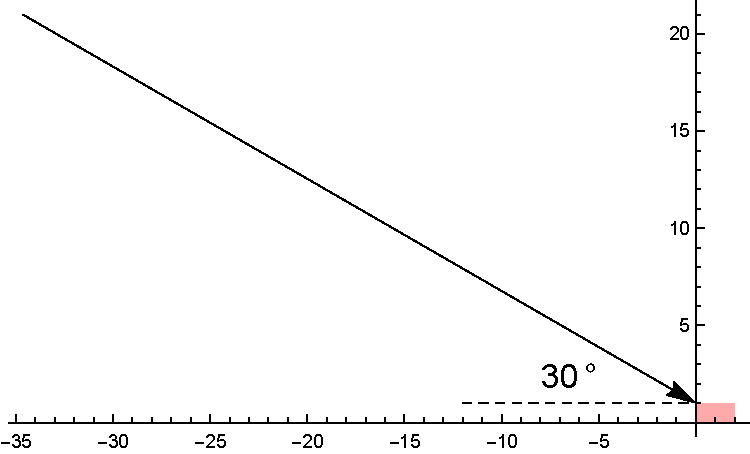
\includegraphics[scale=0.4]{2-2}
\end{figure}

The force is $\vec F$ = 40 ($\cos (-30^\circ), \sin (-30^\circ)$) = (34.6 N, -20 N).

\vspace{\baselineskip}

\noindent
\textbf{2-3} A block is dragged up an inclined plane of slope angle $20^\circ$
by a force \textbf{F} making an angle of $30^\circ$ with the plane.\newline
a) How large a force \textbf{F} is necessary in order that the component $F_x$
parallel to the plane shall be 16 N?\newline
b) How large will the component $F_y$ be? Solve graphically, letting 1 cm = 2 N.

The fact that we're on an incline doesn't matter here, because the problem is asking
for the components parallel ($F_x$) and perpendicular ($F_y$) to the plane.
We know that $F_x$ = F $\cos 30^\circ$ = 16, so F = $\frac{16}{\cos 30^\circ}$ = $18.5$.

Here's the diagram:

\begin{figure}[h]
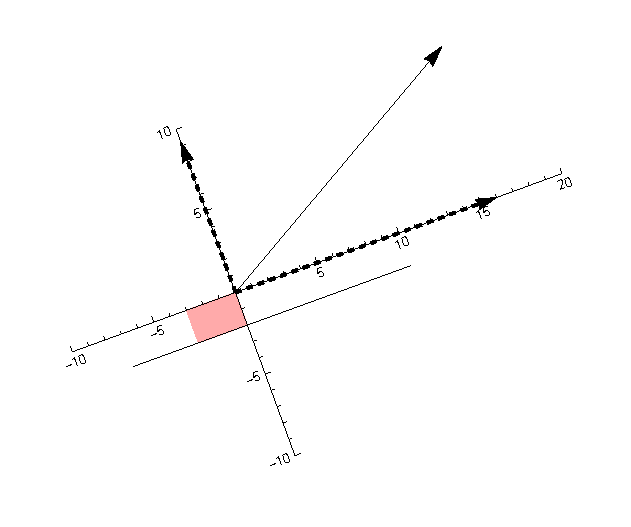
\includegraphics[scale=0.6]{2-3}
\end{figure}

Given the magnitude and direction of the force, we calculate the component perpendicular
to the plane as $F_y$ = $18.5 \sin 30^\circ$ = 9.2 N.

\vspace{\baselineskip}

\noindent
\textbf{2-4} The three forces show in Fig.\,1-14 (of the book) act on a body located at the origin.\newline
a) Find the x- and y-components of each of the three forces.\newline
b) Use the method of rectangular resolution to find the resultant of the forces.\newline
c) Find the magnitude and direction of a forth force that must be added to make the resultant force zero.
Indicate the fourth force by a diagram.

\clearpage
The original diagram is as follows:

\begin{figure}[h]
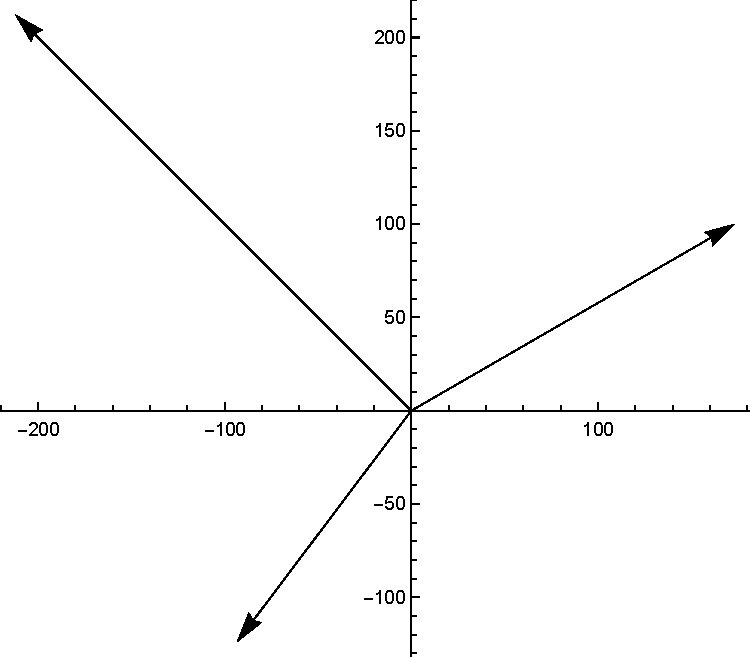
\includegraphics[scale=0.4]{2-4a}
\end{figure}

For the first vector (in quadrant 1), its components are $200\,(\cos 30^\circ, \sin 30^\circ)$ = (173.2, 100.0).
For the second vector (in quadrant 2), the components are $300\,(\cos 135^\circ, \sin 135^\circ)$ = (-212.1, 212.1).
For the third vector (in quadrant 3), the components are $155\,(\cos 233^\circ, \sin 233^\circ)$ = (-93.3, -123.8).

The diagram of the vectors as a polygon is:

\begin{figure}[h]
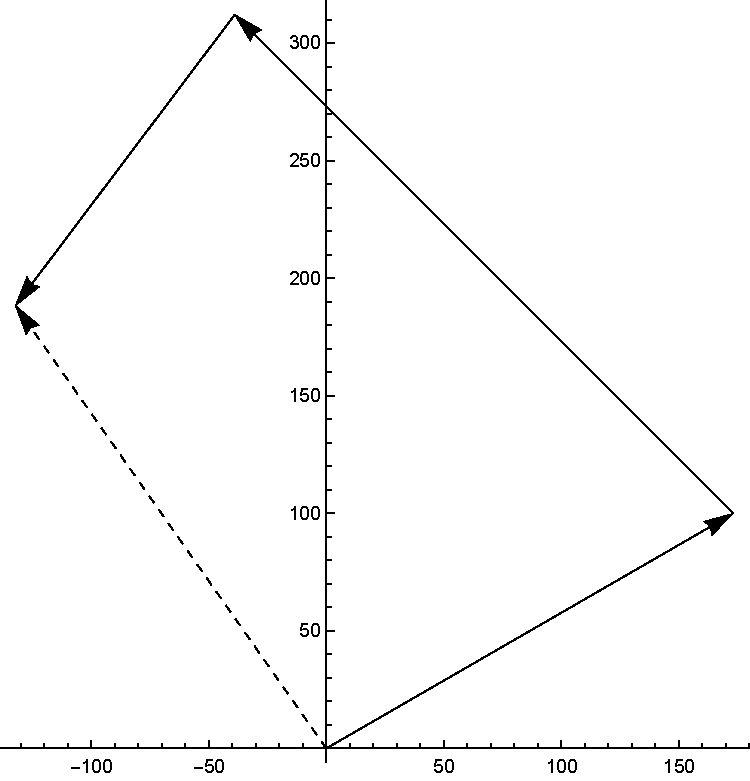
\includegraphics[scale=0.4]{2-4b}
\end{figure}

We get the resultant by adding the components of the vectors.
The x-component is 173.2 - 212.1 - 93.3 = -132.2, and the y-component is 100.0 + 212.1 - 123.8 = 188.3.
The magnitude is $\sqrt{(-132.2)^{2} + (188.3)^2} = 230.1$,
and the direction is $\arctan (-132.2, 188.3) = 125.1^\circ$ (same as $54.9^\circ$ above the -x-axis).

To make the total net force 0, we would just need a fourth vector to point in the opposite direction
from the resultant of the other three vectors.  That vector would have a magnitude of 230.1,
and a direction of $-54.9^\circ$.

\clearpage
The previous diagram becomes:

\begin{figure}[h]
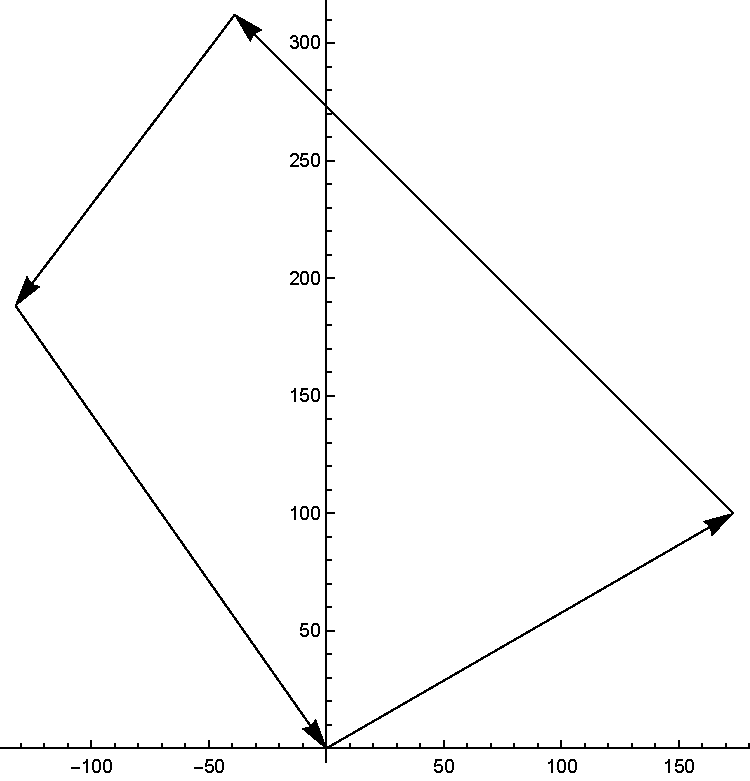
\includegraphics[scale=0.4]{2-4c}
\end{figure}

With the fourth vector, the original diagram becomes:

\begin{figure}[h]
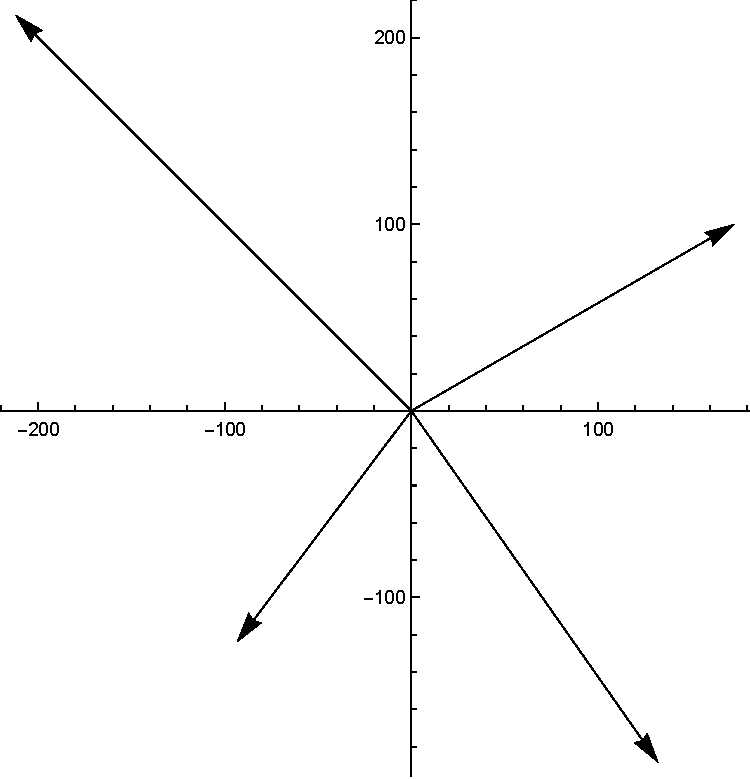
\includegraphics[scale=0.4]{2-4d}
\end{figure}

\vspace{\baselineskip}
\noindent
\textbf{2-5} Use the method of rectangular resolution to find the resultant of the following
set of forces and the angle it makes with the positive x-axis: 200 N, along the x-axis toward the right;
300 N, $60^\circ$ above the x-axis to the right; 100 N, $45^\circ$ above the x-axis to the left;
200 N, along the negative y-axis.

\clearpage
A diagram of the forces is as follows:

\begin{figure}[h]
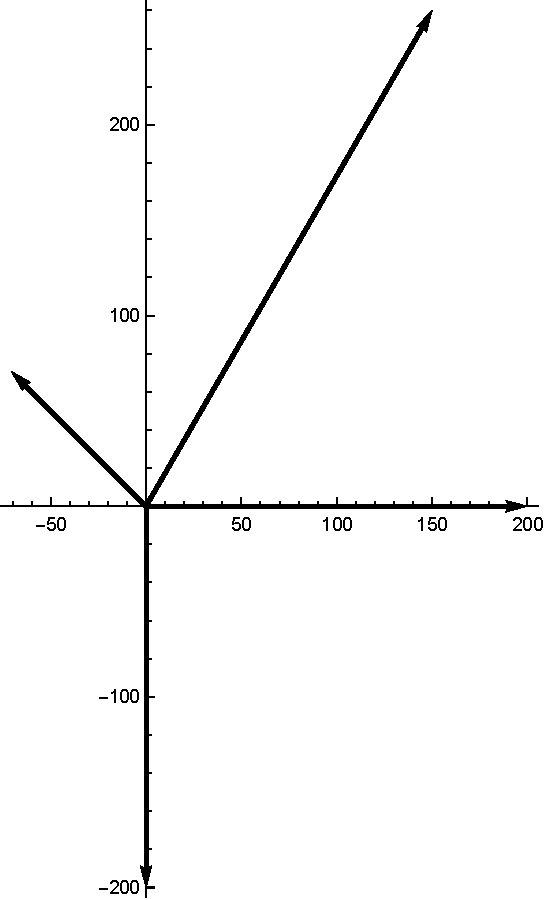
\includegraphics[scale=0.4]{2-5a}
\end{figure}

And here's a diagram of the forces arranged head-to-tail, along with the resultant:

\begin{figure}[h]
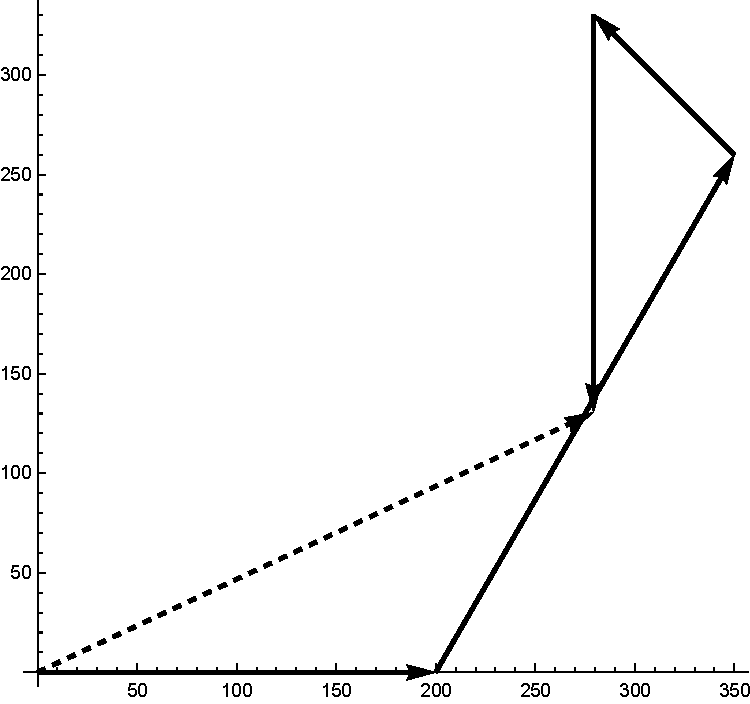
\includegraphics[scale=0.4]{2-5b}
\end{figure}

We derive the components of the resultant by summing the components of the original forces.
The x-component is $200 + 300 \cos 60^\circ + 100 \cos 135^\circ + 0$ = 279.3,
and the y-component is $0 + 300 \sin 60^\circ + 100 \sin 135^\circ - 200$ = 130.5.
The magnitude is $\sqrt{279.3^2 + 130.5^2}$ = 308.3 N, and the direction is
$\arctan (279.3, 130.5) = 25^\circ$.

\vspace{\baselineskip}
\noindent
\textbf{2-6} The resultant of four forces is 1000 N in the direction $30^\circ$ west of north.
Three of the forces are 400 N, $60^\circ$ north of east; 200 N, south; and 400 N, $53^\circ$ west of south.
Find the rectangular components of the fourth force.

\clearpage
Here is a diagram of the forces (the dashed vector is the resultant, and the dotted vector is the fourth force):

\begin{figure}[h]
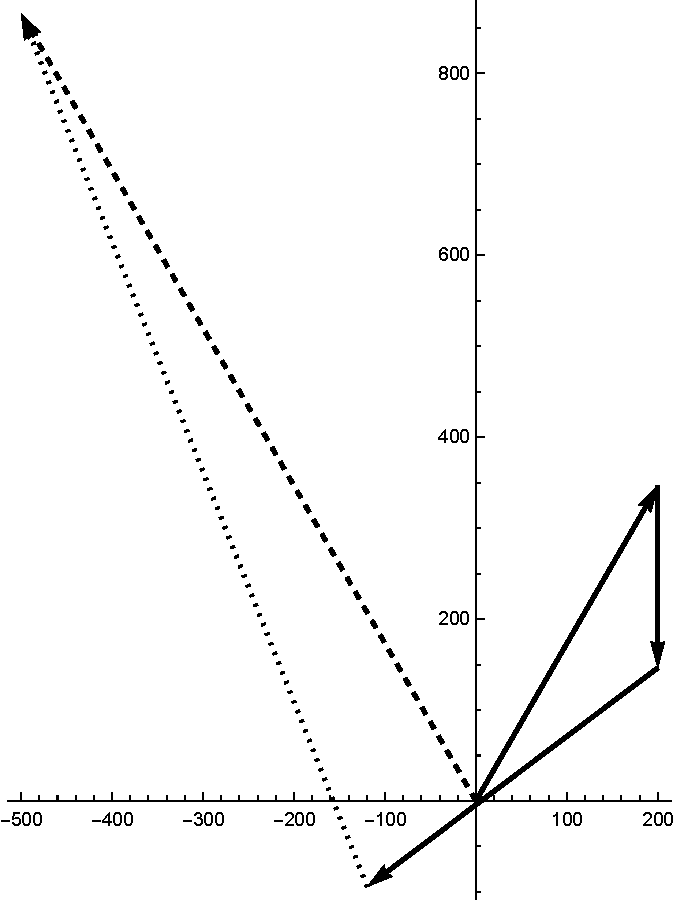
\includegraphics[scale=0.4]{2-6}
\end{figure}

The forth force is the difference between the resultant and the other three forces.
Its x-component is $1000 \cos 120^\circ - 400 \cos 60^\circ - 0 - 400 \cos 217^\circ$ = -380.5,
and its y-component is $1000 \sin 120^\circ - 400 \sin 60^\circ - (-200) - 400 \sin 217^\circ$ = 960.3.

\vspace{\baselineskip}
\noindent
\textbf{2-7} Two forces, $\textbf{F}_1$ and $\textbf{F}_2$, act at a point.
The magnitude of $\textbf{F}_1$ is 8 N, and its direction is $60^\circ$ above the x-axis in the first quadrant.
The magnitude of $\textbf{F}_2$ is 5 N and its direction is $53^\circ$ below the x-axis in the fourth quadrant.\newline
a) What are the horizontal and vertical components of the resultant force?\newline
b) What is the magnitude of the resultant?\newline
c) What is the magnitude of the vector difference $\textbf{F}_1$ - $\textbf{F}_2$?

Here's a diagram of the forces and their resultant:

\begin{figure}[h]
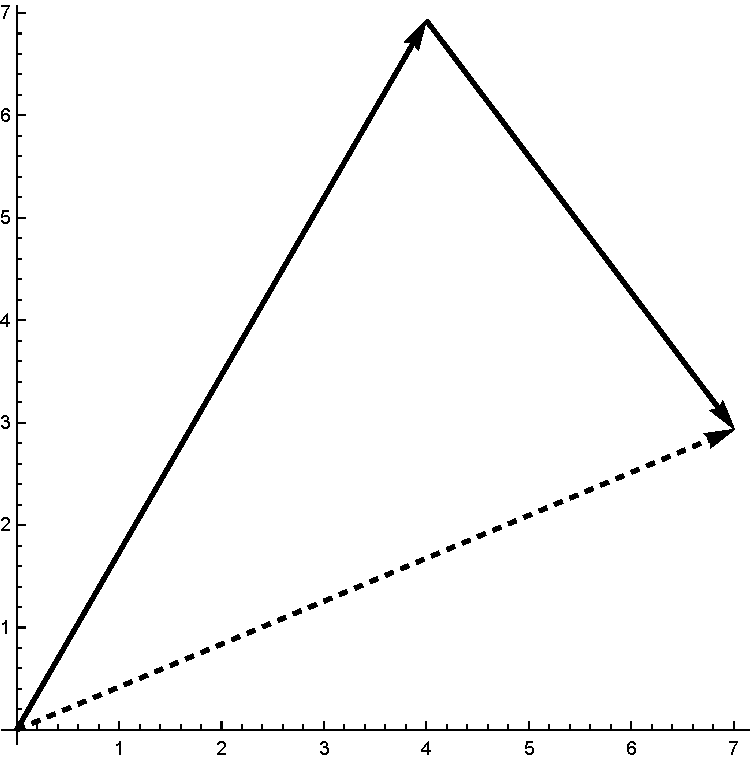
\includegraphics[scale=0.4]{2-7}
\end{figure}

The components of the resultant are the sum of the components of the vectors.
For the x-component, that's $8 \cos 60^\circ + 5 \cos (-53^\circ)$ = 7.01,
and for the y-component, that's $8 \sin 60^\circ + 5 \sin (-53^\circ)$ = 2.94.

The magnitude is $\sqrt{7.01^2 + 2.94^2}$ = 7.60.

\clearpage

Here's a diagram of the difference of the forces (in this case, we arrange the forces tail-to-tail):

\begin{figure}[h]
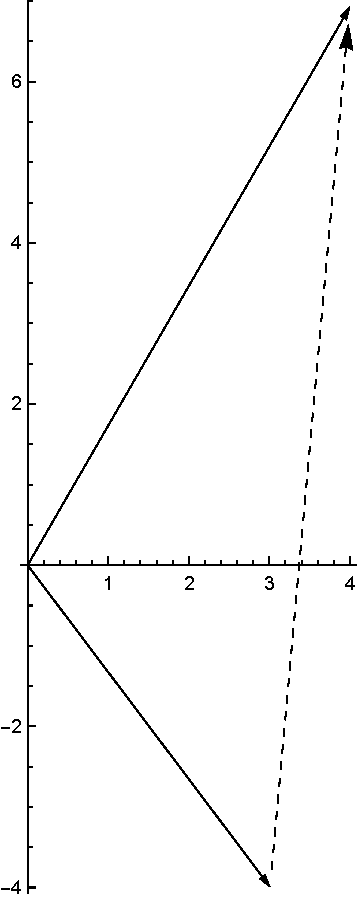
\includegraphics[scale=0.4]{2-7b}
\end{figure}

The components of the difference vector are $8 \cos 60^\circ - 5 \cos (-53^\circ)$ = 1.0 and
$8 \sin 60^\circ - 5 \sin (-53^\circ)$ = 10.9.
The magnitude is $\sqrt{1.0^2 + 10.9^2}$ = 11.0.

\vspace{\baselineskip}
\noindent
\textbf{2-8} Two forces, $\textbf{F}_1$ and $\textbf{F}_2$, act upon a body in such a manner
that the resultant force \textbf{R} has a magnitude equal to that of $\textbf{F}_1$ and
makes an angle of $90^\circ$ with $\textbf{F}_1$.
Let $F_1$ = R = 10 N.  Find  the magnitude of the second force, and its direction
(relative to $\textbf{F}_1$).

The forces form a right triangle:

\begin{figure}[h]
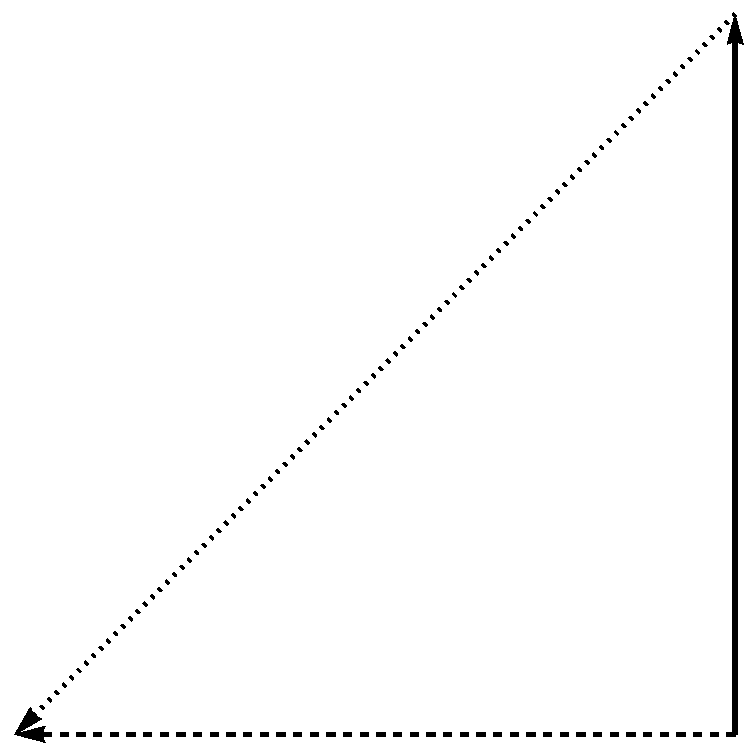
\includegraphics[scale=0.3]{2-8}
\end{figure}

The force we're looking for, $\textbf{F}_2$, is the hypotenuse of the triangle,
so its magnitude is $\sqrt{10^2 + 10^2}$ = $10\sqrt{2}$.
The interior angle is $45^\circ$, so relative to $\textbf{F}_1$ that would be $90^\circ + 45^\circ = 135^\circ$.

The relationship among the forces is \textbf{R} = $\textbf{F}_1$ + $\textbf{F}_2$,
so we could calculate $\textbf{F}_2$ as \textbf{R} - $\textbf{F}_1$ = (-10,0) - (0,10) = (-10,-10).
The magitude is $\sqrt{(-10)^2+(-10)^2} = 10\sqrt{2}$,
and the direction is $\arctan(-10,-10)$ = $225^\circ$.

\vspace{\baselineskip}
\noindent
\textbf{2-9} Two men and a boy want to push a crate in the direction marked $x$ in Fig. 2-15 (of the book).\
The two men push with forces $\textbf{F}_1$ and $\textbf{F}_2$ whose magnitudes and directions are indicated
in the figure.
Find the magnitude and direction of the smallest force that the boy should exert.

\clearpage
The situation is as follows:

\begin{figure}[h]
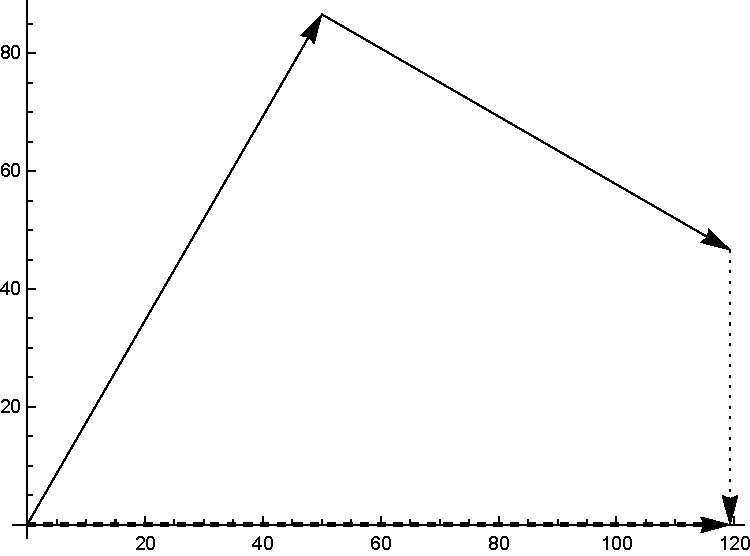
\includegraphics[scale=0.4]{2-9}
\end{figure}

We need for the boy to contribute a force such that its downward component makes the y-component
of the resultant equal to 0.  His force could also include a positive x-component
(in principle, it could include a negative x-component, though that would be counter-productive),
but we are asked to find the minimum force, so he only needs to push in the (negative) y-direction.

The y-component of the boy's force is $0 - F_{1y} - F_{2y}$ = $0 - 100 \sin 60^\circ - 80 \sin (-30^\circ)$ = -46.6.
So the magnitude is 46.6 N, and the direction is $-90^\circ$.

\vspace{\baselineskip}
\noindent
\textbf{2-10} Two men pull horizontally on ropes attached to a post,
the angle between the ropes being $45^\circ$.
If man A exerts a force of 300 N and man B a force of 200 N,
find the magnitude of the resultant force and the angle is makes with A's pull.  Solve:\newline
a) graphically, using a scale diagram (let 1 cm = 500 N), and\newline
b) analytically, using components.

Here's the diagram:

\begin{figure}[h]
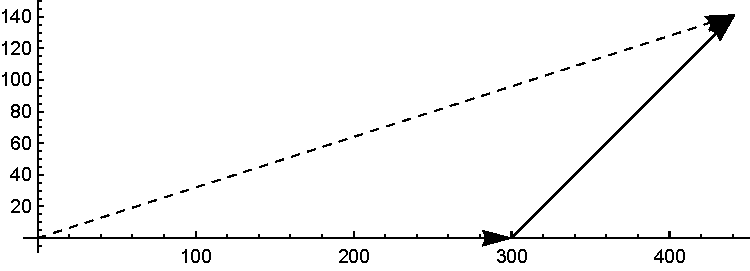
\includegraphics[scale=0.4]{2-10}
\end{figure}

The resultant is the sum of the forces, so that's \textbf{R} = $\textbf{F}_A$ + $\textbf{F}_B$ =
(300,0) + $200 (\cos 45^\circ, \sin 45^\circ)$ = (441.4, 141.4).  The magnitude is
$\sqrt{441.4^2 + 141.4^2}$ = 463.5\,N, and the direction is $\arctan (441.4, 141.4)$ = $17.8^\circ$.

\vspace{\baselineskip}
\noindent
\textbf{2-11} Imagine that your are holding a book weighting 4\,N at rest on the palm of your hand.
Complete the following sentences.\newline
a) A downward force of magnitude 4\,N is exerted on the book by \underline{the earth}.

\textit{This is just the weight of the book, due to the force of gravity.}

\noindent
b) An upward force of magnitude \underline{4\,N} is exerted on \underline{the book} by the hand.

\textit{This is just a normal force, the same as if the book were on a table or something.}

\noindent
c) Is the upward force (b) the reaction to the downward force (a)?

\textit{No.  Action-reaction pairs are always between the same two objects.  The earth pulls the book down,
and the book pulls the earth up.}

\noindent
d) The reaction to force (a) is a force of magnitude \underline{4\,N},
exerted on \underline{the earth} by \underline{the book}.
Its direction is \underline{upward}.

\textit{The force on the book by the earth, and the force on the earth by the book, form a third-law pair.}

\noindent
e) The reaction to force (b) is a force of magnitude \underline{4\,N}, exerted on \underline{the hand}
by \underline{the book}.  Its direction is \underline{downward}.

\textit{The force on the book by the hand, and the force on the hand by the book, form a third-law pair.}

\noindent
f) That the forces (a) and (b) are equal and opposite is an example of Netwon's \underline{first law}.

\textit{The net force on the book is zero, so the book in equilibrium.  Newton's first law says that if
there is no net force on an object, then it will continue doing what it's doing.
Here that means the book stays at rest.}

\noindent
g) That forces (b) and (e) are equal and opposite is an example of Newton's \underline{third} law.

\textit{The third law always applies to the same pair of objects.  Here that's the book and the hand.}

\vspace{\baselineskip}
\noindent
Suppose now that you exert an upward force of magnitude 5\,N on the book.\newline
h) Does the book remain in equilibrium?

\textit{No, because now the net force on the book is positive, so the book accelerates upward.}

\noindent
i) Is the force exerted on the book by the hand equal and opposite to the force exerted on the book by the earth?

\textit{No, because these are independent forces.  The earth continues to exert the same downward force on the book.}

\noindent
j) Is the force exerted on the book by the earth equal and opposite to the force exerted on the earth by the book?

\textit{Yes.  The book and earth form a third-law pair.
That interaction is independent of the interaction between the book and the hand.}

\noindent
k) Is the force exerted on the book by the hand equal and opposite to the force exerted on the hand by the book?

\textit{Yes.  The book and the hand form a third law pair.}

\vspace{\baselineskip}
\noindent
Finally, suppose that you snatch your hand away while the book is moving upward.\newline
l) How many forces then act on the book?

\textit{There is only one force, the downward force due to gravity.}

\noindent
m) Is the book in equilibrium?

\textit{No, because the net force on the book is no longer zero.  The acceleration is negative,
because the force is acting in the direction opposite the direction of motion, so the book slows down.}

\noindent
n) What balances the downward force exerted on the book by the earth?

\textit{Nothing balances it, because it's the only force acting on the book.
The book is decelerating, so Newton's second law is, er, in force.}

\vspace{\baselineskip}
\noindent
\textbf{2-12} A block is given a push along a tabletop, and slides off the edge  of the table.\newline
a) What forces are exerted on it while it is falling from the table to the floor?\newline
b) What is the reaction to each force, that is, on what body and by what body is the reaction exerted?
Neglect air resistance.

The only force acting on the book once it falls off the table is the force of gravity.

The book and earth form a third law pair.
The earth exerts a force on the book (causing the book to fall, with increasing speed, towards the earth),
and the book exerts a force on the earth.

\vspace{\baselineskip}
\noindent
\textbf{2-13} Two 10-N weights are suspended at opposite ends of a rope that passes over a light
frictionless pulley.  The pulley is attached to a chain that goes to the ceiling.\newline
a) What is the tension in the rope?\newline
b) What is the tension in the chain?

Consider one of the weights.  The weight is in equilibrium, so the upward tension in the rope must have the same magnitude
as the downward force of gravity.  Therefore the tension in the rope must be 10\,N.  In a rope (without friction)
the tension is everywhere the same, so this analysis applies to the other weight as well.

The pulley is stationary so it is also in equilibrium.  There are two downward forces acting on the pulley
(from the tension on both halves of the rope), and there is the upward force from the chain.
These opposing forces have the same magnitude, so the tension in the chain is the sum of the tensions
from the rope, which is 20\,N.

\vspace{\baselineskip}
\noindent
\textbf{2-14} In figure 2-16 (of the book), a man lifts a weight $w$ by pulling down on a rope with force F.
The upper pulley is attached to the ceiling by a chain, and the lower pulley is attached to the weight by another chain.
If $w$ = 400\,N, find the tension in each chain and the force F is the weight is lifted at constant speed.
Assume the weights of the rope, pulleys, and chain to be negligible.

The weight is moving at constant speed, so the net force must be 0.  The upward tension in the chain from the lower pulley
to which the weight is attached has the same magnitude as the downward force of gravity, so its tension must be 400\,N.

The sum of the tension from both halves of the rope to which the lower pulley is attached must have the same magnitude
as the downward force from the chain (to which the weight is attached), so tension in the rope must be 200\,N.

The tension in a rope is everywhere the same, so the downward force F must also have magnitude 200\,N.

For the upper pulley, the upward tension in the chain attached to the ceiling equals the sum of the downward tension from
both halves of the rope, so the tension in the chain must be 400\,N.

If we were to treat the pulleys as an opaque system, moving upward at constant speed, then the upward
forces acting on the system must have the same magnitude as the downward forces acting on the system.
Here the upward forces on the system are from the rope attached to the ceiling (200\,N),
and from the chain attached to the ceiling (400\,N), for a total of 600\,N.
The downward forces on the system are from the man pulling down on the rope with force F (200\,N),
and from the weight attached to the lower pulley (400\,N), for a total of 600\,N.
So we have done the correct accounting of all the forces acting on the system.

Note that even though the man is able to lift a 400\,N weight using only 200\,N of force,
there is no free lunch.  To move the weight up by one unit of distance, he must move the lower pulley up
by one unit, but it requires two units of rope to do so.
The work done on the weight to lift it by 1\,m is 400\,N $\cdot$ 1\,m = 400\,J.
The work done by the man on the rope is 200\,N $\cdot$ 2\,m = 400\,J,
so we have also correctly accounted for the work.

\vspace{\baselineskip}
\noindent
\textbf{2-15} In Fig. 2-9a (of the book), let the weight of the hanging block be 50\,N.\newline
a) Find the tension in each cord.\newline
b) If the $60^\circ$ angle is changed to $45^\circ$, find the tension in each cord.

The system is in equilibrium, so when we decompose each force, the magnitudes of the components must be equal.
Considering the forces on the mass, the tension $T_1$ must equal the mass's weight, so $T_1$ = 50\,N.
(Another way to see this is to remember that the purpose of a rope is to transmit a force.
If the weight of the mass attached to the rope is 50\,N, then that's also the tension in the rope.)

Considering the forces at the knot,
we have
$T_1 = T_3 \cdot \sin 60^\circ$, so $T_3 = \frac{50}{\sqrt{3}/2}$ $\approx$ 57.7\,N,
and $T_2 = T_3 \cdot \cos 60^\circ = \frac{50}{\sqrt{3}}$ $\approx$ 28.9\,N.

If we change the angle to $45^\circ$, then $T_1 = T_3 \cdot \sin 45^\circ$,
so $T_3 = \frac{50}{1/\sqrt{2}}$ $\approx$ 70.7\,N,
and $T_2 = T_3 \cdot \cos 45^\circ = 50\,N$.
(Tension $T_1$ equals the weight, so it doesn't change.)

\vspace{\baselineskip}
\noindent
\textbf{2-16} A picture frame is hung against a wall, suspended by two wires
attached to its upper corners.
If the two wires make the same angle with the vertical,
what must this angle be for the tension in each wire to equal the weight of the frame?

The picture frame is in equilibrium, so the sum of the upward components of the tension in the wires
must equal the downward weight of the frame.  So we have $T \cos \theta + T \cos \theta = w$.
We are told that the tension in each wire equals the weight, so $2\,w \cos \theta = w$,
which simplifies to $\cos \theta = \frac{1}{2}$, and therefore $\theta = 60^\circ$.

\vspace{\baselineskip}
\noindent
\textbf{2-17} Figure 2-17 (in the book) shows a technique call rappelling, used by mountaineers
for descending vertical rock faces.
The climber sites in a rope seat, and the rappel rope passes through a friction device attached
to this seat.
Suppose the rock is perfectly smooth, and the climber's feet push horizontally into the rock;
if the climber's weight is 800\,N, find the tension in the rope and the force his fee exert
on the rock face.

The system is in equilibrium so opposing forces must have the same magnitude.
Let $T_1$ be the tension in the rope.  The upward component $T_1$ must equal the downward
weight of the climber, so we have $T_1 cos 15^\circ$ = 800\,N,
and therefore $T_1$ = $\frac{800}{\cos 15^\circ}$ $\approx$ 828.2\,N.

The tension of the rope pulls the climber into the rock face with a force of $T_1 \sin 15^\circ$
$\approx$ 214.4\,N.

\vspace{\baselineskip}
\noindent
\textbf{2-18} Figure 2-18 (of the book) illustrates a mountaineering technique call a Tyrolean traverse.
A rope is stretched tightly between two points, and the climber slides across the rope.
The climber's weight is 800\,N, and the breaking strength of the rope (typically nylon, 11 mm diameter)
is 20,000\,N.\newline
a) If the angle $\theta$ is $15^\circ$ , find the tension in the rope.\newline
b) What is the smallest value the angle $\theta$ can have if the rope is not to break?

The sum of the upward components of the tension in the two halves of the rope equals the downward
weight of the climber.  We have $T \sin 15^\circ + T \sin 15^\circ$ = 800\,N,
so $T = \frac{800}{2 \sin 15^\circ}$ = 1545.5\,N.

For the system to be in equilibrium, it's always the case that the upward component of the tension
in the rope equals the weight of the climber, no matter what is the angle.
Increasing the tension will make the angle smaller, but the upward component will always be the same.
The relationship is $T = \frac{800}{2 \sin \theta}$.
The maximum tension is 20,000\,N, so we can write this as
$\theta$ = $\arcsin(\frac{800}{2 \cdot 20,000})$ = $1.15^\circ$.

\vspace{\baselineskip}
\noindent
\textbf{2-19} A man proposes to pull his car out of a mudhole on a country road by stretching a rope
between the front of his car and a solid object directly in front of the car, and then pushing sideways
at the midpoint of the rope.
Suppose that the rope is 50\,m long, and that a sideways force of 300\,N is required to displace
the midpoint sideways 5\,m.
Determine the tension in the rope and the forward component of force on the car.

We interpret the problem statement to mean that the distance between the solid object and the car
is 50\,m, and that by applying a crosswise force to the rope that this stretches it a bit.
The half-distance (25\,m) to the object, and the 5\,m crosswise displacement, makes a triangle,
with the rope as the hypotenuse, having length $\sqrt{25^2 + 5^2}$ = $\sqrt{650}$.

Let $\theta$ be the angle formed between the direct line from the car to the object and the rope.
This gives us $\sin \theta = \frac{5}{\sqrt{650}}$, and $\cos \theta = \frac{25}{\sqrt{650}}$.

Let T be the tension in the rope.
Each half of the rope from the midpoint makes a separate contribution to the force,
so we have $2 \cdot T \sin \theta = 300$.
That gives us $T = \frac{300}{2 \cdot \frac{5}{\sqrt{650}}}$ = 764.9\,N.

The force pulling the car forward is $T \cos \theta$ = $764.9 \cdot \frac{25}{\sqrt{650}}$ = 750\,N.

\vspace{\baselineskip}
\noindent
\textbf{2-20} Find the tension in each cord in Fig.\,2-19 if the weight of the
suspended body is 200\,N.

For part (a), the sum of upward components of the cords equals the weight of the object.
The sideways components have opposite directions but are equal in magnitude.
So we have $A \sin 30^\circ + B \sin 45^\circ = 200$, and
$A \cos 30^\circ - B \cos 45^\circ = 0$.
That gives us two equations and two unknowns.
Solving this system of equations yields A = 146.4\,N and B = 179.3\,N.
The tension in cord C equals the weight of the object, so C = 200\,N.

For part (b), the upward component of B equals the weight of the object,
which gives us $B = \frac{200}{\sin 45^\circ}$ = 282.8\,N.
The sideways component of B equals the tension in A,
so we have $A = B \cos 45^\circ$ = 200\,N.
The tension in C is the same as the weight of the object, 200\,N.

For part (c), the vertical component of cord A is downward,
in the same direction as the weight.
The angle that A makes with the horizonal is $30^\circ$.
For the vertical forces, we have $B \sin 45^\circ = A \sin 30^\circ + 200$.
For the horizontal forces, we have $B \cos 45^\circ = A \cos 30^\circ$.
Solving this system of equations yields A = 546.4\,N and B = 669.2\,N.
As in the other systems, cord C is 200\,N.

For part (d), the vertical components of the C cords equals the weight
of the object.  So that's $2 \cdot C \sin 53^\circ = 200$,
so $C = \frac{200}{2 \sin 53^\circ}$ = 125.2\,N.
To determine A, we have a couple of options.
In the first case, the vertical component of A equals the vertical component of C,
which gives us the relation $A \sin 37^\circ = C \sin 53^\circ$.
Solving for A that way gives us $A = C \cdot \frac{\sin 53^\circ}{\sin 37^\circ}$ = 166.2\,N.
Alternatively, we could treat the tension in cords B and C as internal forces
(which would make them uninteresting),
and realize that the upward components of A equal the downward weight of the object.
That relation is $2 \cdot A \sin 37^\circ = 200$.
Solving for A yields the same answer.

At the point where cords A, B, and C meet, the system is in equibrium.
The horizonal component of A equals the sum of the tension from B
and the horizonal component of C.
That relation is $A \cos 37^\circ = B + C \cos 53^\circ$.
We have calculated A and C,
so that yields $B = A \cos 37^\circ - C \cos 53^\circ$ = 57.3\,N.

\vspace{\baselineskip}
\noindent
\textbf{2-21} In Fig.\,2-20 (of the book), find the weight of the suspended body if the
tension in the diagonal string is 20\,N.

The point where the diagonal string meets the rightward force and downward weight is
in equilibrium, so the sum of the forces must be zero.
The downward weight of the body is balanced by the vertical
component of the tension in the diagonal string.
That value is $20 \sin 45^\circ = \frac{20}{\sqrt{2}}$ = 14.1\,N.

\vspace{\baselineskip}
\noindent
\textbf{2-22} In each of the arrangements of Fig.\,2-21 (of the book),
find each tension and the weight of the suspended body if the indicated
tension T is 10\,N.

For part (a), since the sum of the interior angles is $180^\circ$,
the angle between the ceiling and the indicated rope (T=10\,N) is $60^\circ$.
For the horizontal forces, we have $10 \cos 60^\circ$ = $T_2 \cos 30^\circ$,
so $T_2 = \frac{10 \cos 60^\circ}{\cos 30^\circ}$ = 5.77\,N.
For the vertical forces, we have w = $10 \sin 60^\circ + 5.77 \sin 30^\circ$ = 11.5\,N.

For part (b), we are given the lengths, so we must compute the angles.
Call $\alpha$ the angle between the ropes of length 3 and 6, and $\beta$ the angle
between the ropes of length 4 (marked with T=10\,N) and 6.
From the law of cosines, we have $\cos \alpha$ = $\frac{29}{36}$,
and $\cos \beta$ = $\frac{43}{48}$.  (We need not evaluate the actual angles,
since it's the $\cos$ and $\sin$ values that we care about.)
The relation between the horizontal forces is $T_2 \cos \alpha = 10 \cos \beta$,
which gives us $T_2 = \frac{10 \cdot 43/48}{29/36}$ = 11.1\,N.

From the law of sines we have $\sin \alpha$ = $\frac{4}{3} \sin \beta$.
We need one more equation, so we use the fact that $\cos^2 \beta + \sin^2 \beta = 1$.
This gives us $\sin \beta = \sqrt{1-\cos^2 \beta} = \sqrt{1-(43/48)^2}$.
The weight equals the sum of the upward components of the tension in each rope,
so we have w = $11.1 \sin \alpha + 10 \sin \beta$ = $11.1 \frac{4}{3} \sin \beta + 10 \sin \beta$ =
$(11.1 \frac{4}{3} + 10) \sqrt{1-(43/48)^2}$ = 11.0\,N.

\vspace{\baselineskip}
\noindent
\textbf{2-23}\newline
a) Block A in Fig.\,2-22 (of the book) weighs 100\,N.
The coefficient of static friction between the block and the surface on which it rests
is 0.30.  The weight $w$ is 20.0\,N and the system is in equilibrium.
Find the friction force exerted on block A.\newline
b) Find the maximum weight $w$ for which the system will remain in equilibrium.

For part (a) we are told the weight, and must find the friction force.
Static friction is a constraint force, so it will adjust as necessary (up to a limit)
to keep the system in equilibrium.
Call $T_A$ the tension in the rope connected to block A,
and $T_B$ the tension in the diagonal rope connected to the wall.
The downward force of the weight equals the upward component of $T_B$,
$w = T_B \sin 45^\circ$.  The tension $T_A$ equals the horizontal component
of $T_B$, $T_A = T_B \cos 45^\circ = \frac{w}{\sin 45^\circ} \cdot \cos 45^\circ = w$.
Block A is in equilibrium, so the resistive force of the static friction equals the tension
of rope, $f_A = T_A = w$ = 20\,N.

For part (b) we are asked to derive the maximum weight such that the system remains in equilibrium.
The force of static friction will adjust as the weight changes, up the limit of $\mu F_N$
(after which block A begins to slip and kinetic friction applies).
Block A is in equilibrium,
so the normal force $F_N$ equals the weight of the block, 100\,N.
That gives us $f_{max} = \mu F_N = 0.3 \cdot 100$ = 30\,N = $T_A = T_B \cos 45^\circ$.
The maximum weight is therefore $w = T_B \sin 45^\circ = \frac{30}{\cos 45^\circ} \cdot \sin 45^\circ$ = 30\,N.

\vspace{\baselineskip}
\noindent
\textbf{2-24} A block hangs from a cord 10\,m long.
A second cord is tied to the midpoint of the first,
and a horizontal pull equal to half the weight of the block is exerted on it,
the second cord being always kept horizontal.\newline
a) How far will the block be pulled to one side?\newline
b) How far will it be lifted?

When the second cord is first pulled (to the right, say), there is no other horizontal force,
so the system is not in equilibrium, and the point of intersection moves (accelerated) up and to the right.
The first cord is attached to the ceiling, and forms angle $\theta$ with the ceiling.
Gradually the horizontal component of the tension in the first cord (directed to the left)
equals the horizonal tension in the second cord,
and the vertical component of the tension (directed upward)
equals the weight of the block,
so the system returns to equilibrium.

Call T the tension in the first cord, attached to the ceiling.
The relationship between the horizontal forces is $T \cos \theta = w/2$,
and between the vertical forces, $T \sin \theta = w$.
If we divide these equations, we have $\frac{\sin \theta}{\cos \theta}$ = 2,
which gives us $\theta = \arctan 2$.

The upper part of the first cord (oriented diagonally) forms the hypotenuse of a triangle.
Its horizontal leg is the displacement of the lower part of the cord from its original position,
which is $5 \cos \theta$ = 2.24\,m.

The block was lifted by the difference between the old height of the midpoint
and its new height (the vertical leg of the triangle),
$5 - 5 \sin \theta$ = 0.528\,m.

\vspace{\baselineskip}
\noindent
\textbf{2-25} A flexible rope of weight $w$ hangs between two hooks at the same height,
as shown in Fig.\,2-23 (of the book).
At each end the rope makes an angle $\theta$ with the horizonal.\newline
a) What is the magnitude and direction of the force \textbf{F} exerted by the rope
on the hook at the left?\newline
b) What is the tension \textbf{T} in the rope at its lowest point?

The system is in equilibrium, so the magnitude of the force pulling the rope up must
equal the weight pulling the rope down.
The tension force, by the rope on the hook, has a direction tangent to the curve of the rope,
so on the left the tension is directed down and to the right.
Per Newton's third law, there is a reaction force, by the hook on the rope,
which is directed up and to the left.
If the force is \textbf{F}, then the magnitude of its upward component is $F \sin \theta$.
There are two hooks, so we have $2\,F \sin \theta = w$.
The force is therefore $F = \frac{w}{2\,\sin \theta}$.

The tension is tangent to the curve of the rope, so at the lowest point, the tension is horizontal.
The system is in equilibrium, so the magnitude of the (horizontal) tension at the lowest point
must equal the horizonal component of the force of the hook on the rope.
So we have $T = F \cos \theta = \frac{w}{2\,\sin \theta} \cdot \cos \theta = \frac{w}{2\,\tan \theta}$.

\vspace{\baselineskip}
\noindent
\textbf{2-26} A 30-N block is pulled at constant speed up a frictionless inclined plane by a weight
of 10\,N hanging from a cord attached to the block and passing over a frictionless
pulley at the top of the plane.  (See Fig 2-10 of the book.) Find\newline
a) the slope angle of the plane,\newline
b) the tension in the cord, and\newline
c) the normal force exerted on the block by the plane.

The block is moving at constant speed, so there is no acceleration and hence the system
is in equilibrium.  The magnitude of the upward tension in the rope is equal to
the downward force of the 10-N weight, so the tension in the cord is 10\,N.

There is no friction in the pulley, so the tension in the rope is everywhere the same,
and therefore the force pulling the 30-N block up the plane is 10\,N.
This must equal the magnitude of the component of the 30-N weight directed down the plane,
so we have $30 \sin \theta = 10$ and therefore $\theta = \arcsin (1/3) \approx 19.5^\circ$.

The normal force pushing against the 30-N block equals the component of the 30-N weight
that is perpendicular to the plane, so its magnitude is
$30 \cos \theta$ = $30 \cos (\arcsin (1/3)) \approx 28.3\,N$.

\vspace{\baselineskip}
\noindent
\textbf{2-27}\newline
a) A block rests upon a rough horizontal surface.
A horizontal force $T$ is applied to the block and is slowly increased from zero.
Draw a graph with $T$ along the x-axis and the friction force $f$ along the y-axis,
starting at $T = 0$ and showing the region of no motion, the point where motion impends,
and the region where motion exists.\newline
b) A block of weight $w$ rests on a rough horizontal plank.
The slope angle of the plank $\theta$ is gradually increased until the block starts to slip.
Draw two graphs, both with $\theta$ along the x-axis.
In one graph show the ratio of the normal force to the weight

Assume that the weight of the block is 10\,N, and that the coefficient of static friction is 0.4,
and for kinetic friction it's 0.1.
Static friction is a constraint force, so it adjusts, up to the limit $\mu_s \cdot \textbf{N}$ =
$0.4 \cdot 10$ = 4\,N.
As the tension is increased from 0 to 4\,N, the static friction increases by the same amount.
These forces are in opposition so the net force is zero and hence there is no motion.
Here's the diagram for part (a):

\begin{figure}[h]
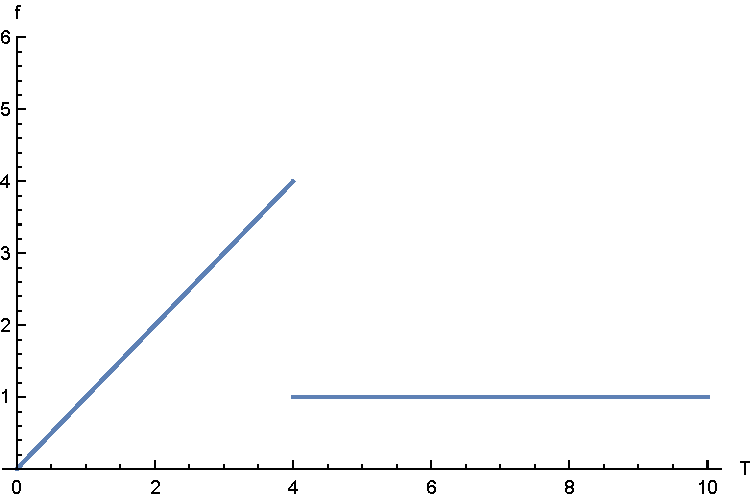
\includegraphics[scale=0.4]{2-27a}
\end{figure}

However, when the tension is 4\,N we have reached the limit of static friction and the block
slips.  The block is now moving, so we have (constant) kinetic friction,
equal to $\mu_k \cdot \textbf{N}$ = $0.1 \cdot 10$ = 1\,N.
Beyond a tension of 4\,N there is a non-zero net force, and the block accelerates.

For part (b), we have a block on a plane whose incline varies.
The normal force on the block equals the component of the weight that is perpendicular the plane,
$w \cos \theta$.  Here's that diagram:

\clearpage
\begin{figure}[h]
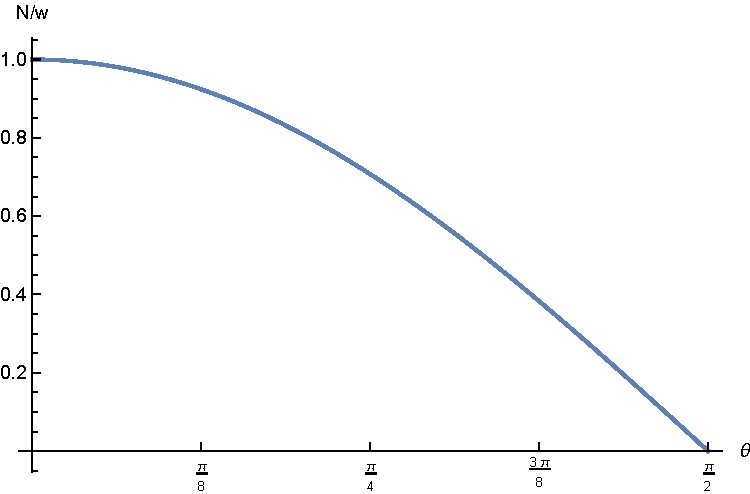
\includegraphics[scale=0.4]{2-27c}
\end{figure}

When the plank is not inclined, the normal force equals the weight.  However, as $\theta$ is increased,
the normal force decreases, reaching its limiting value when $\theta = 90^\circ$, at which
point the block is in free fall and there is no normal force at all.

The component of the weight that points down the plane is $w \sin \theta$.
The force of static friction, which points up the plane, varies up to the limit
of $\mu_s \cdot w\,\cos \theta$.
As $\theta$ is increased, the downward force eventually equals the maximum static friction force
and we have $w \sin \theta = \mu_s \cdot w \cos \theta$, and so the block begins to slip when $\tan \theta = \mu_s$.
Here's the diagram:

\begin{figure}[h]
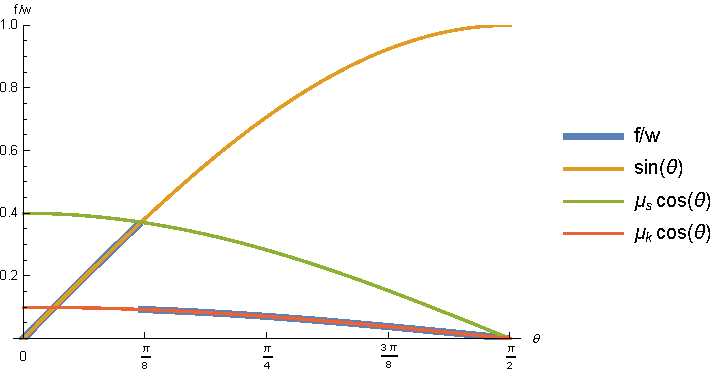
\includegraphics[scale=0.6]{2-27b}
\end{figure}

The blue curve is the ratio of the friction force to the weight.
You can see that it tracks the force down the plane due to the weight (the orange curve).
The downward force and the static friction force are the same, up until the point when the downward force
equals the limiting value of the static friction force (the green curve), when the block begins to slip.
Beyond that point, the block is sliding down the plane and so we have kinetic friction (the red curve).

Note that as $\theta$ increases, the ratio of the force down the plane and the weight approaches 1 (the orange curve).
At the limiting value of $\theta = 90^\circ$, the block is in free fall and the force down the plane is
the same as the weight.  The normal force approaches 0, and so when the block is in free fall, there is
no normal force and hence no friction (the green and red curves).

\vspace{\baselineskip}
\noindent
\textbf{2-28} A block weighing 20\,N rests on a horizontal surface.
The coefficient of static friction between block and surface is 0.40
and the coefficient of sliding friction is 0.20.\newline
a) How large is the friction force exerted on the block?\newline
b) How great will the friction force be if a horizontal force of 5\,N is exerted on the block?\newline
c) What is the minimum force that will start the block in motion?\newline
d) What is the minimum force that will keep the block in motion once is has been started?\newline
e) If the horizontal force is 10\,N, how great is the friction force?

Friction is a force that resists motion.  In order to move the object (which is initially at rest),
we would have to apply a force.  But there is no force (in the horizontal direction),
so there is no friction, so the friction force is 0.
(Note that we can have no motion and non-zero friction.  The point is that the friction force
is a reaction to some other force.  With no other force, there is no reaction, hence no friction.)

Static friction is a constraint force, so it adjusts up to a limit,
equal to $\mu_s F_N$ = $0.40 \cdot 20$ = 8\,N.
Below the limit, the static friction force adjusts such that it always equals the external force applied to the block,
so the friction force is 5\,N.

To move the block we must apply a force equal to the limit of static friction, which is 8\,N in this case.

Once the block is moving, we have sliding friction equal to $\mu_k F_N$ = $0.20 \cdot 20$ = 4\,N.
So to keep the block moving, we would need a force at least equal to 4\,N.

If the external force is 10\,N we are above the limit of static friction,
so sliding friction applies.  Sliding friction is constant, so its value is 4\,N.


\vspace{\baselineskip}
\noindent
\textbf{2-29} A block is pulled to the right at constant velocity by a 10-N force
acting $30^\circ$ above the horizontal.
The coefficient of sliding friction between the block and the surface is 0.5.
What is the weight of the block?

In order to compute the magnitude of the sliding friction force, we must determine
the normal force.  The normal force is a constraint force, so it adjusts in order
to keep the block in equilibrium.  The upward forces acting on the block are
the normal force and the vertical component of the pull force.  Since the block
is in equilibrium we know the sum of these forces must equal the weight.
So we have $F_N + 10 \sin 30^\circ = w$ and therefore $F_N = w - 5$.

The sliding friction is $\mu_k F_N$ = $0.5 \cdot (w - 5)$.  The block is being
pulled at constant velocity, so the block is in equilibrium and
the sliding friction must equal the horizontal component of the pull force,
which gives us $0.5 \cdot (w - 5) = 10 \cos 30^\circ$.
Solving for w yields 22.3\,N.


\vspace{\baselineskip}
\noindent
\textbf{2-30} A block weighing 14\,N is placed on an inclined plane and connected
to a 10-N block by a cord passing over a small frictionless pulley, as in Fig. 2-10 (of the book).
The coefficient of sliding friction between the block and the plane is $\left( \frac{1}{7} \right)$.
For what two values of $\theta$ will the system move with constant velocity?
(Hint: $\cos \theta = \sqrt{1-\sin^2 \theta}$.)

The block can be moving up the ramp or down the ramp.
The friction force is directed opposite the direction of motion, so if the block is moving up the plane,
then the friction force is directed down the plane, and vice versa.

The normal force equals the component of the block's weight that is perpendicular to the plane,
so that's $14 \cos \theta$.  Sliding friction is constant, with value $\mu_k F_N$ =
$\frac{1}{7} \cdot 14 \cos \theta$ = $2 \cos \theta$.

The weight of the block has a component parallel the plane, directed down the plane,
having magnitude $14 \sin \theta$.  The rope transmits the weight of the 10-N block
(and the pulley changes the direction of the tension),
so the tension in the cord attached to the 14-N block is 10\,N.

If the block is moving up the plane at constant speed, the system is in equilibrium
and we have $14 \sin \theta + 2 \cos \theta = 10$,
which gives us $\theta = 2 \arctan (1/3) = 36.9^\circ$.

If the block is moving down the plane at constant speed,
then we have $14 \sin \theta = 2 \cos \theta + 10$,
which gives us $\theta = 2 \arctan (1/2) = 53.1^\circ$.

\vspace{\baselineskip}
\noindent
\textbf{2-31} A block weighing 100\,N is placed on an inclinded plane of slope angle $30^\circ$
and is connected to a second hanging block of weight $w$ by a cord passing over a small
frictionless pulley, as in Fig. 2-10.
The coefficient of static friction is 0.40 and the coefficient of sliding friction is 0.30.\newline
a) Find the weight $w$ for which the 100-N block moves up the plane at constant speed.\newline
b) Find the weight $w$ for which it moves down the plane at constant speed.\newline
c) For what range of values of $w$ will the block remain at rest?

For part (a), the block is moving up the plane, so the friction force is directed down the plane.
The system is in equilibrium (because the block is moving at constant speed),
so the component of the block's weight directed down the plane, plus the downward-directed friction force,
equals the tension in the rope, which is itself equal to the weight of the other block, $w$.
That gives us $100 \sin 30^\circ + 0.3 \cdot 100 \cos 30^\circ = w$, so $w$ = 80.0\,N.

For part (b), the block is moving down the plane, so the friction force is directed up the plane.
The component of the block's weight, directed down the plane, equals the sum of the tension in the rope
plus the friction force, both directed up the plane.
This gives us $100 \sin 30^\circ = 0.3 \cdot 100 \cos 30^\circ + w$, so $w$ = 24.0\,N.

Static friction is a constraint force, that adjusts up to a limit, to prevent relative motion.
Part (c) is similar to parts (a) and (b) but with kinetic friction replaced with static friction.
The maximum weight of the second block before slippage occurs up the plane corresponds to the
limit of static friction (directed down the plane), so we have
$100 \sin 30^\circ + 0.4 \cdot 100 \cos 30^\circ = w$, so $w$ = 84.6\,N.
The minimum weight of the second block before slippage occurs down the plane corresponds
to the limit of static friction (directed up the plane), so we have
$100 \sin 30^\circ = w + 0.4 \cdot 100 \cos 30^\circ$, and therefore $w$ = 15.4\,N.

\vspace{\baselineskip}
\noindent
\textbf{2-32} What force P at an angle $\phi$ above the horizontal is needed to drag
a box of weight $w$ at constant speed along a level floor if we are given that the
coefficient of sliding friction between box and floor is $\mu$?

The normal force on the weight is a constraint force, so it adjusts as necessary to keep the weight
in (vertical) equilibrium.
The sum of the normal force and the vertical component of the pull force equals the weight,
which gives us $F_N + P \sin \phi = w$, so $F_N = w - P \sin \phi$.

We need the know the normal force in order to determine the friction force.
The block is moving at constant speed, so the horizontal forces are in equilibrium.
We have $P \cos \phi = \mu F_N = \mu (w - P \sin \phi)$,
which gives us P = $\frac{\mu w}{\mu \sin \phi + \cos \phi}$.

\vspace{\baselineskip}
\noindent
\textbf{2-33} A safe weighing 2000\,N is to be lowered at constant speed down skids
4\,m long, from a truck 2\,m high.\newline
a) If the coefficient of sliding friction between safe and skids is 0.30,
will the safe need to be pulled down or held back?\newline
b) What is the coefficient of sliding friction?

To determine whether we need to pull the safe down the ramp, or hold it back,
we need to compare the component of the weight down the incline to the friction force
up the incline.

The value of the incline is $\sin \theta = \frac{2}{4}$, which implies that the angle is $30^\circ$.
The component of the weight parallel to the ramp is $2000 \sin 30^\circ$ = 1000\,N.
The friction force is $\mu_k F_N$ = $0.3 \cdot 2000 \cos 30^\circ$ $\approx$ 520\,N.
For the weight to be in equilibrium, the force down the ramp must equal the force up the ramp.
The friction force is less than downward component of the weight, so we must hold the weight back
to make up the difference, by applying a force equal to $1000 - 520$ = 480\,N.


\vspace{\baselineskip}
\noindent
\textbf{2-34}\newline
a) If a force of 86\,N parallel to the surface of a $20^\circ$ inclined plane will push
a 120-N block up the plane at constant speed, what force parallel to the plane will push
it down at constant speed?\newline
b) What is the coefficient of sliding friction?

If we're pushing the block up the plane, the friction force is directed down the plane.
The system is in equilibrium, so we have $120 \sin 20^\circ + \mu_k \cdot 120 \cos 20^\circ = 86$.
That gives us $\mu_k$ = 0.399.

If we're pushing the block down the plane (call it force F), then the friction force is directed up the plane,
so $120 \sin 20^\circ + F = \mu_k \cdot \cos 20^\circ$, so F = 3.92\,N.

\vspace{\baselineskip}
\noindent
\textbf{2-35} Block A in Fig.\,2-24 weighs 4\,N and block B weighs 8\,N.
The coefficient of sliding friction between all surfaces is 0.25.
Find the force \textbf{P} necessary to drag block B to the left at constant speed\newline
a) if A rests on B and moves with it,\newline
b) if B is held at rest, and\newline
c) if A and B are connected by a light flexible cord passing around a fixed frictionless pulley.

For part (a), block A moves with block B so only need to consider the friction between block B
and the floor.  The normal force that pushes against the blocks equals the combined weight of both blocks,
which is 12\,N.  The friction force is therefore $\mu_k F_N$ = $0.25 \cdot 12$ = 3\,N.
The block is in equilibrium with the pull force, so P = 3\,N.

In part (b), block A is attached to the wall, so there is relative motion between A and block B,
and we must consider the friction force between B and A and between B and the ground.
The friction force between B and the ground is the same as in part (a), so that's 3\,N.
The friction force due to block A is $\mu_k F_{N,A}$ = $0.25 \cdot 4$ = 1\,N.
The block is in equilibrium, so the pull force equals the total friction, P = 4\,N.

In part (c) the cord to which block A is attached is in tension with block B,
so this tension is another rightward force on block B.
The friction force of block A on B forms a third-law pair with the friction force
of block B on A (which points to the left).  Block A is in equilibrium,
so this gives us the value of the tension in the cord, 1\,N.
The pull force on B is the sum of the friction forces and the tension,
which gives us P = 5\,N.

\vspace{\baselineskip}
\noindent
\textbf{2-36} Block A, of weight $w$, slides down an inclined plane S
of slope angle $37^\circ$, at constant velocity while the plank B,
also of weight $w$, rests on top of A.
The plank is attached by a cord to the top of the plane (Fig.\,2-25).\newline
a) Draw a diagram of all the forces acting on block A.\newline
b) If the coefficient of kinetic friction is the same between surfaces A and B
and between S and A, determine its value.

The horizontal forces that act on block A are the component of the weight directed
down the ramp, and the friction from block B and from surface S.
The vertical forces include the component of the weight perpendicular to the plane,
and the normal forces from block B and surface S.
The diagram is as follows:

\begin{figure}[h]
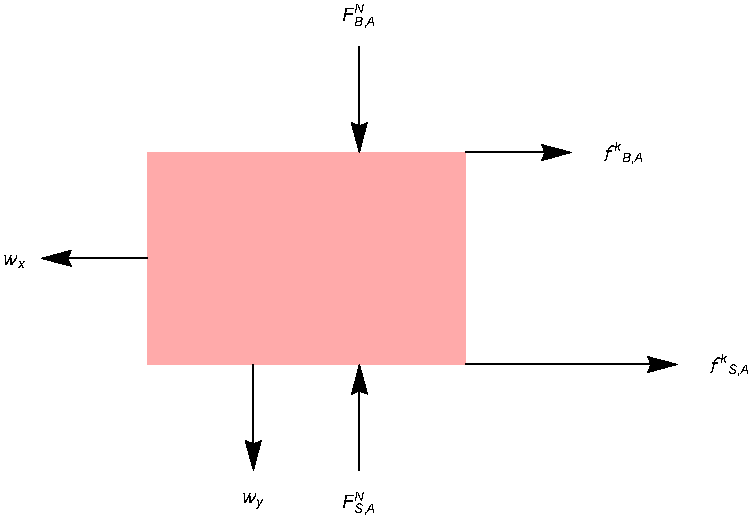
\includegraphics[scale=0.6]{2-36}
\end{figure}

The normal force of B on A equals the perpendicular component of B's weight.
That makes B's friction force $\mu_k F^{N}_{B,A}$ = $\mu_k \cdot w \cos 37^\circ$.
The normal force from the surface equals the perpendicular component of both blocks,
so S's friction force is $\mu_k F^{N}_{S,A}$ = $\mu_k \cdot 2 w \cos 37^\circ$.
The total friction is $\mu_k \cdot 3 w \cos 37^\circ$.

The system is in equilibrium, so the component of the A's weight down the ramp equals
the friction forces up the ramp, so we have $w \sin 37^\circ = \mu_k \cdot 3 w \cos 37^\circ$.
That gives us $\mu_k = \frac{1}{3} \tan 37^\circ$ = 0.251.

\vspace{\baselineskip}
\noindent
\textbf{2-37} Two blocks, A and B, are placed as in Fig.\,2-26 and connected by ropes to block C.
Both A and B weight 20\,N and the coefficient of sliding friction between each block and the
surface is 0.5.
Block C descends with constant velocity.\newline
a) Draw two separate force diagrams showing the forces acting on A and on B.\newline
b) What is the weight of block C?

\clearpage
The forces acting on block A include the tension and friction (in the horizontal direction)
and the weight and normal forces (in the vertical direction).
Here's the force diagram for block A:

\begin{figure}[h]
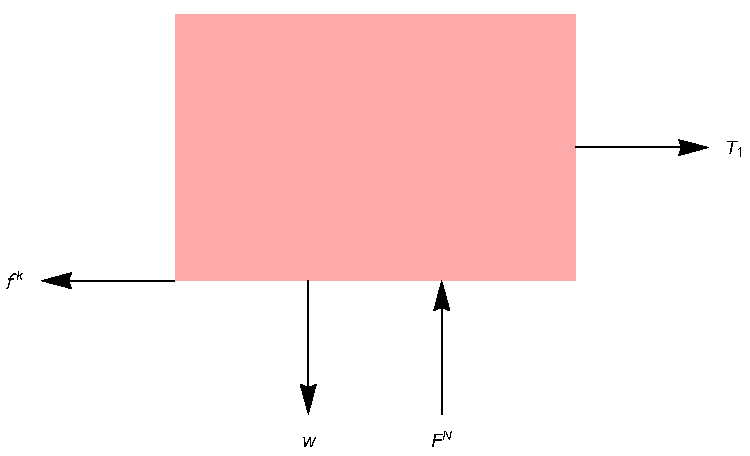
\includegraphics[scale=0.6]{2-37a}
\end{figure}

The forces acting on block A include the tension from both cords, the friction,
and the component of the weight directed down the ramp,
and the component of the weight in the direction perpendicular to the ramp
and the normal force.  Here's the diagram for block B:

\begin{figure}[h]
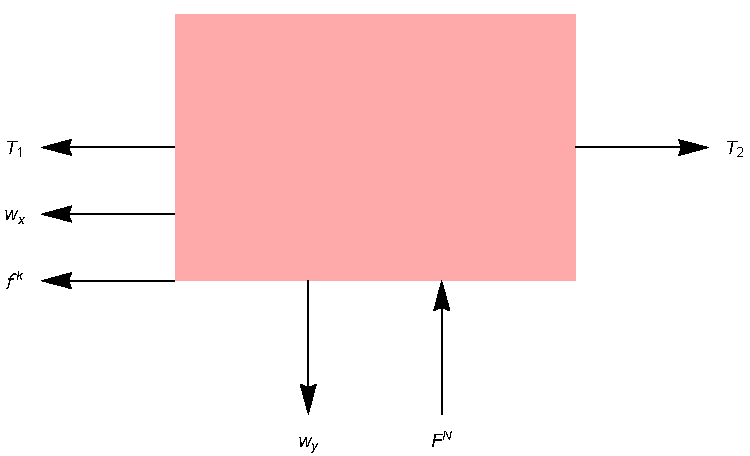
\includegraphics[scale=0.6]{2-37b}
\end{figure}

We are told that block C is descending with constant velocity,
so the system is in equilibrium and opposing forces have equal magnitude.
The normal force acting on block A equals its weight, 20\,N.
The tension equals the friction, so we have $T_1$ = $\mu_k F_N$ = $0.5 \cdot 20$ = 10\,N.

Block C is in equilibrium, so its weight, $w$, equals the tension in the cord to which it is connected.

The friction force acting on block B is $\mu_k F_N$ = $0.5 \cdot 20 \cos 37^\circ = 10 \cos 37^\circ$.
The horizontal forces are related by $w = 10 + 20 \sin 37^\circ + 10 \cos 37^\circ$ = 30.0\,N.

\vspace{\baselineskip}
\noindent
Study Guide - Chapter 2 Quiz

\vspace{\baselineskip}
\noindent
\textbf{1} A horizontal rope is stretched between two buildings 20\,m apart.
When a man weighing 800\,N hangs from the center of the rope, the center is 4\,m
lower than the ends.
What is the tension in the rope?

The man is supported by the tension in both halves of the rope.
Each half of the rope forms a triangle, with the rope as the hypotenuse,
the horizonal leg equal to half the distance between the buildings (10\,m),
and the vertical leg equal to 4\,m.
The length of the hypotenuse is $\sqrt{4^2 + 10^2}$ = $\sqrt{116}$.
Let $\theta$ be the angle formed by the hypotenuse and the horizontal leg;
then $\sin \theta = \frac{4}{\sqrt{116}}$.

The system is in equilibrium, so the upward components of the tension in the rope
equal the downward weight of the man, giving us $2\,T \sin \theta = 800$,
so T = $\frac{800}{2 \sin \theta} = 400 \cdot \frac{\sqrt{116}}{4}$ = 1077\,N.

Note that the answer given in the study guide, 1081\,N, is incorrect.
It appears that the authors first evaluated the sine value,
$\sin \theta$ = $\frac{4}{\sqrt{116}}$ = 0.3714, but then rounded this down to 0.37.
They computed their result as $\frac{400}{0.37}$ = 1081\,N, but this value is
too large.  If you carry 4 digits of precision, then $\frac{400}{0.3714}$ gives
you the correct answer of 1077\,N.

\vspace{\baselineskip}
\noindent
\textbf{2} Two ropes attached to the ceiling support a 100\,N weight.
One rope makes an angle of $30^\circ$ with the ceiling and the other
makes an angle of $45^\circ$ with the ceiling.
Find the tension in each rope.

The system is in equilibrium, so the horizontal forces sum to zero as
do the vertical forces.
Let $T_1$ be the tension in the rope that is $30^\circ$ from the ceiling,
and $T_2$ be the tension in the rope that is $45^\circ$ from the ceiling.
The horizontal components are related by $T_1 \cos 30^\circ = T_2 \sin 45^\circ$.
The upward components of the ropes equal the downward weight, which is
$T_1 \sin 30^\circ + T_2 \sin 45^\circ = 100$.
This is two equations in two unknowns, so we have $T_1$ = 73.2\,N, and $T_2$ = 89.7\,N.

% 2018-08-06

\clearpage

%TODO(matthewjheaney): chap 3

\end{document}
